\documentclass[../notas medios.tex]{subfiles}
\begin{document}

\chapter{Análisis de Tensiones}

\graphicspath{{img/Cap3/}} 								 % Specifies the directory where pictures are stored
\section{Introducción}
%
En la sección introductoria se presentaron algunas ideas simples que permitían
pasar del problema discreto (modelo de partículas) al continuo (modelo de puntos
materiales). En términos generales, se planteaba la conversión de las ecuaciones
gobernantes representativas de principios físicos propuestos a nivel de la
partícula a ecuaciones de campo mediante un proceso de homogenización.

En esta sección se particulariza el problema al caso de la Mecánica Newtoniana
para sistemas de muchas partículas, dando como resultado el concepto de tensión
el cual resulta ser una cantidad de tipo tensorial (descrita ahora por 3
vectores indicando la distribución de fuerzas a lo largo de 3 direcciones). 

%Como producto final de la presente sección se dispondrá entonces de las
%ecuaciones gobernantes y condiciones de frontera en términos de fuerza. El
%problema de valores en la frontera resultante solo será soluble una vez
%involucremos los cambios de configuración y su relación con las fuerzas a través
%de leyes constitutivas (es decir relaciones tensión-deformación).

Al final de esta sección el estudiante deberá estar en la capacidad de:

\begin{itemize}
\item[•] Reconocer los tipos de fuerzas presentes en el modelo de los medios continuos.
\item[•] Reconocer en el concepto de esfuerzo (o fuerza por unidad de superficie) y en su caracter tensorial una herramienta matemática para describir los cambios de cantidad de movimiento en el modelo del medio continuo.
\item[•] Entender el vector de tracciones como una descripción de las fuerzas por unidad de superficie asociadas con un plano determinado.
\item[•] Determinar las componentes del vector de tracciones en asocio con un plano determinado dado el tensor de esfuerzos en un punto del medio.
\item[•] Transformar de un sistema de referencia a otro las componentes del tensor de esfuerzos.
\item[•] Evaluar condiciones de falla en términos de tensiones a través de un punto del medio continuo. 
\item[•] Identificar los invariantes del tensor de esfuerzos como las descripciones absolutas del estado de tensiones en un punto.
\item[•] Determinar las tensiones extremas y las direcciones en que estas se presentan para un estado de tensiones en 2D y 3D.
\item[•] Calcular los invariantes para estados de tensiones en 2D y 3D.
\item[•] Representar el tensor de tensiones en la orientación principal.
\end{itemize}


\section{Interacciones mecánicas-Origen del concepto de tensión}

En el caso particular del problema mecánico, la \cref{ca_ef_rep} tomada de la sección introductoria

\begin{equation}
f\left( {\frac{{d\beta }}{{dt}}} \right) = \alpha
\label{ca_ef_rep}
\end{equation}

se reduce a la segunda ley de Newton para una partícula de masa $m$, velocidad
$\vec V$, fuerza $\vec F$ y cantidad de movimiento $\vec P = m\vec V$.
Nuevamente estipulamos que en este caso la variable respuesta o efecto $\beta$ 
corresponde a la cantidad de movimiento $\vec P = m\vec V$ y la variable fuente
o causa $\alpha$ que introduce cambios temporales en $\beta$ corresponde a la
fuerza $\vec F$. La ley general de la \cref{ca_ef_rep} válida a nivel de la
partícula se reduce entonces a la segunda ley de Newton que relaciona los
cambios en la cantidad de movimiento y la fuerza como

\begin{equation}
\vec F = \frac{{d\vec P}}{{dt}} \equiv \frac{{dm\vec V}}{{dt}}.
\label{morate}
\end{equation}

Esta ley de carácter discreto\footnote{Discreto significa existente a nivel de
la partícula} indica que la fuerza es el {\bf dispositivo matemático}  que
permite representar cambios de cantidad de movimiento entre una partícula y el
medio ambiente. Claramente identificamos en el concepto matemático de fuerza el
punto de partida del modelo de la {\bf Mecánica de los Medios Continuos}.

\subsection{Fuerzas de cuerpo}
Nuevamente nos apoyaremos en la esquematización de la \cref{infinite} en la cual
se considera un medio infinito que representa {\bf el medio ambiente}. Este se
encuentra acotado por una superficie ${S_\infty }$ encerrando el volumen $B(t)$.
Consideramos además un medio continuo ({\bf el sistema}) localizado al interior
de este espacio infinito y delimitado por una superficie $S(t)$ que acota un volumen $V(t)$
y que se encuentra en contacto directo con el medio ambiente a través de su frontera $S(t)$.


\begin{figure}[H]
\centering
	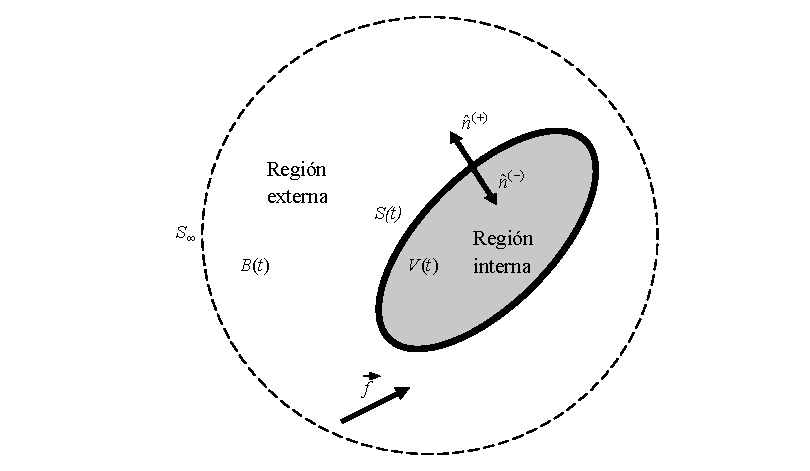
\includegraphics[width=4.0 in]{infinite.pdf}
	\caption{Medio continuo interactuando con un espacio infinito.}
	\label{infinite}
\end{figure}

Utilizaremos la siguiente descripción de las regiones involucradas: La región
localizada del lado positivo del vector normal ${\hat n^{( + )}}$ a $S(t)$ se
denominará en lo que sigue la {\bf región externa}. De manera consistente, la
región localizada del lado negativo del vector normal ${\hat n^{( - )}}$ a
$S(t)$ se denominará la {\bf región interna}.

Se desea entonces caracterizar la interacción mecánica entre las regiones
interna y externa debida a la existencia de una {\bf fuente de cantidad de
movimiento} pero tratada esta como una distribución o función. Se denota allí
esta función como $\vec f$, la cual en lo que sigue equivale a la función
general $\Phi$ y representa una densidad de fuerza (fuerza por unidad de volumen).

Aunque esta densidad se representa en la figura como localizada en un punto se
enfatiza en que la misma puede estar distribuida en todo el volumen incluyendo
la región interna o estar localizada solo en el infinito de la región externa.
En cualquier caso esta fuente es introducida por algún agente externo.

En el primer caso de fuentes internas o una distribución interna de fuerzas por
unidad de volumen decimos que estas son representativas de interacciones a
distancia. Esto significa que el agente externo que las produce no se encuentra
en la vecindad del medio en cuestión. Estos son por ejemplo los campos
gravitacionales o electromagnéticos.

\subsection{Fuerzas de superficie-El vector de tracciones}
De cualquier forma, ya sea que existen fuentes internas o externas se generara
también una interacción a través de la superficie o por contacto directo entre
los dos medios. La \cref{dcl_rep} representa el diagrama de cuerpo libre de la
región interna. En éste se muestran las interacciones $\vec t$ generadas por
contacto directo a través de la superficie $S(t)$ y las interacciones a
distancia $\vec f$, distribuidas estas sobre todo el volumen $V(t)$. La
función vectorial $\vec t$ representa una función o distribución de fuerzas por
unidad de superficie equivalente acá a la interacción por contacto directo entre
las regiones interna y externa. Estas fuerzas en la superficie son necesarias
para mantener la condición de continuidad entre el medio ambiente y el medio continuo.

\begin{figure}[H]
\centering
	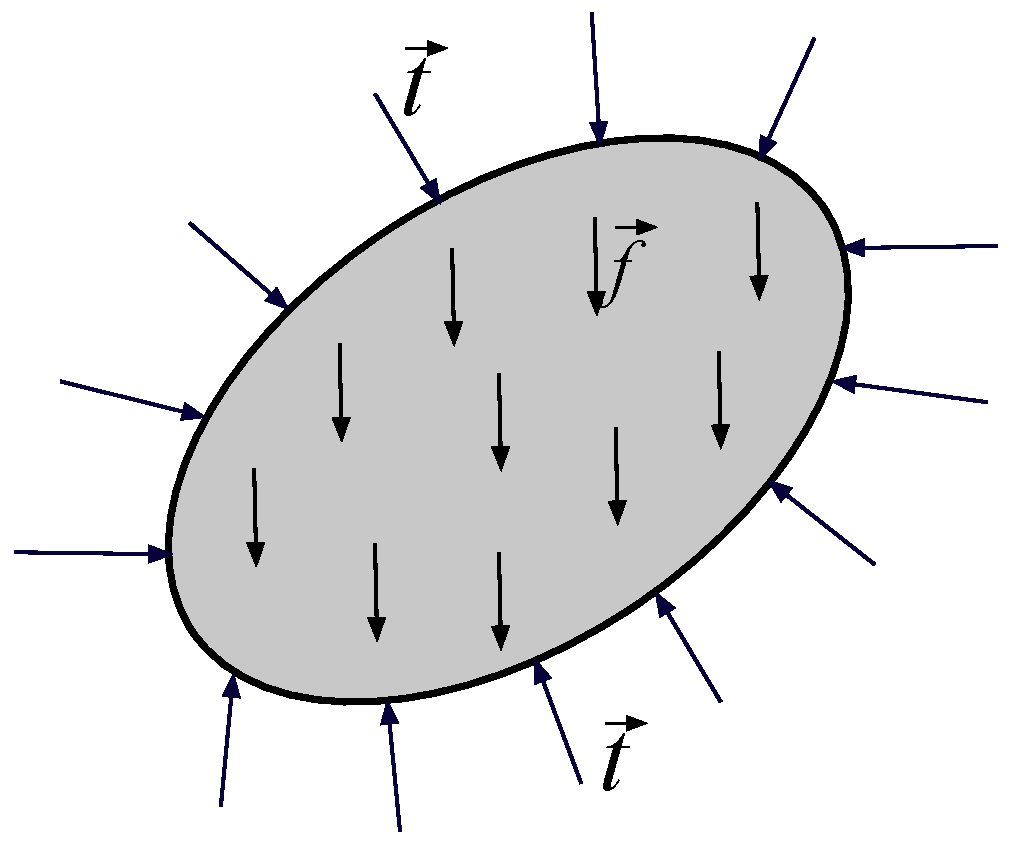
\includegraphics[width=2.8 in]{dcl.pdf}
	\caption{Diagrama de cuerpo libre de la región interna interactuando con la región externa.}
	\label{dcl_rep}
\end{figure}
%
La \cref{dcl_ext} muestra el correspondiente diagrama de cuerpo libe para la
región externa. En esta figura, la función $\vec t$ nuevamente representa la
fuerza por unidad de superficie sobre la superficie $S(t)$ de la región externa
que es igual y opuesta a la función $\vec t$ actuando sobre la superficie $S(t)$
de la región interna (y de acuerdo con el principio de acción y reacción). Estas
fuerzas son equilibradas por una función análoga pero localizada sobre la frontera o superficie ${S_\infty }$.

Nuevamente la función $\vec t$ ha sido construida con fundamento en el continuo
matemático y su definición de estado límite. En el modelo clásico de la mecánica
de los medios continuos el carácter de esta interacción por contacto directo se
encuentra descrito por el primer postulado de Cauchy.  Como tal, este admite
verificación experimental más no demostración matemática.  Se llegará entonces a
un modelo de la mecánica de los medios continuos basado en la definición de fuerzas superficiales de Cauchy.


\begin{figure}[H]
\centering
	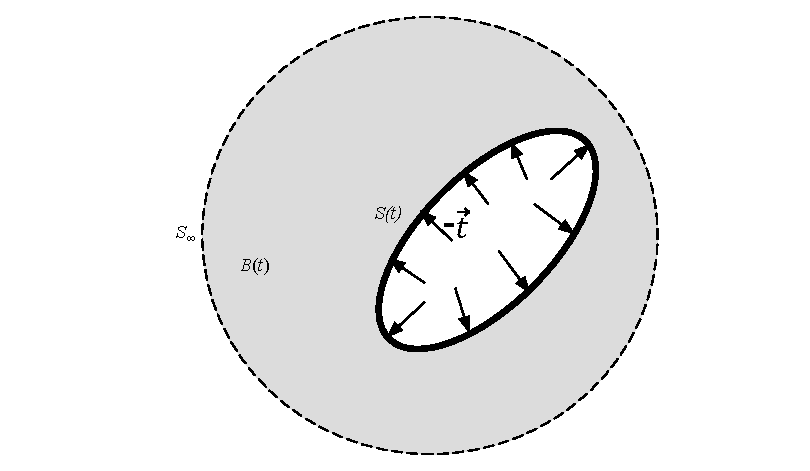
\includegraphics[width=4.0 in]{dcl_ext.pdf}
	\caption{Diagrama de cuerpo libre de la región externa interactuando con la
	región interna.}
	\label{dcl_ext}
\end{figure}

En algunos tratamientos es común encontrar las funciones $\vec f$ y $\vec t$ 
diferenciadas como “fuerzas” externas e internas. Esto es motivado en el hecho
de que las segundas aparecen toda vez que propongamos un nuevo diagrama de
cuerpo libre haciendo cortes o exponiendo nuevas superficies extraídas del
sistema original. Por ejemplo si del volumen $V(t)$ aisláramos un nuevo volumen
$b(t)$, sobre la nueva superficie expuesta aparecería entonces una nueva función
$\vec t$ que efectivamente mantiene unidas las dos porciones resultantes. En
estos términos la distribución $\vec t$ era una fuerza interna antes de realizar
la partición y aparece ahora como una fuerza externa en el nuevo diagrama de
cuerpo libre. En cualquier caso la distribución $\vec t$ aparece para equilibrar
una función fuente externa $\vec f$. En este sentido también consideramos en
este tratamiento a la función $\vec t$ como externa.

Es válido entonces clasificar las fuerzas como {\bf externas} cuando actúan
sobre el sistema y como {\bf internas} cuando actúan entre partes del sistema.
Sin embargo debe aclararse que mediante una elección apropiada de un diagrama de
cuerpo libre extraído del sistema original, cualquier fuerza interna al sistema
original puede exponerse como una fuerza externa.

En este tratamiento denominaremos las fuentes o fuerzas $\vec f$ como {\bf
fuerzas de cuerpo} y las fuerzas $\vec t$ como fuerzas por unidad de superficie
o {\bf tracciones}.
Tratamos ambas como externas con la salvedad de que las primeras son debidas a
agentes externos a distancia mientras que las segundas son debidas a contacto
directo a través de superficies del medio continuo.

\subsubsection{Dependencia del vector de tracciones en la dirección del vector normal}
En lo que sigue se presentará un ejemplo (ver \cref{soil}) aplicado a un caso
particular que pretende servir de abrebocas o justificación para la introducción
de manera formal del primer postulado de Cauchy conducente al concepto matemático de tensión.

\begin{figure}[H]
\centering
	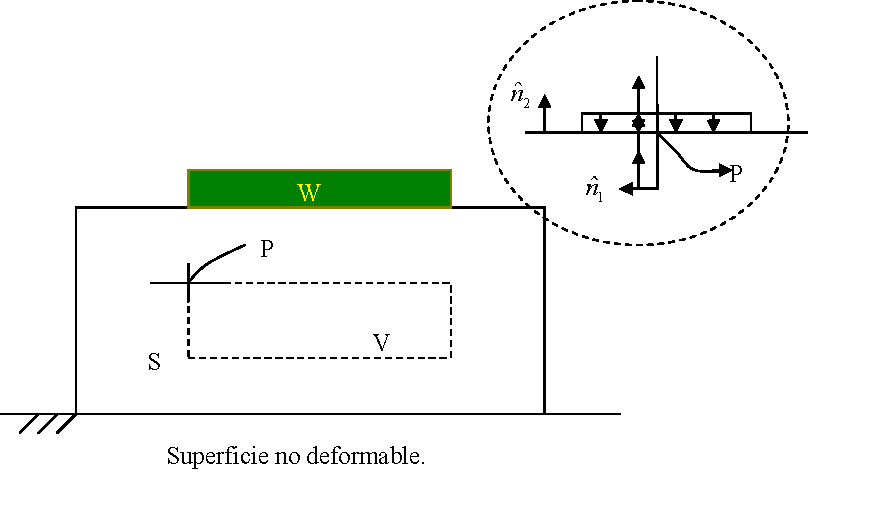
\includegraphics[width=4.0 in]{soil.pdf}
	\caption{Interacción por contacto en un punto P sobre la frontera de un medio continuo de volumen $V$ acotado por la superficie $S$.}
	\label{soil}
\end{figure}

En el ejemplo ilustrado en la \cref{soil} se extrae o aísla para efectos de su
análisis el volumen acotado internamente por la superficie matemática
(abstracta, artificial o virtual) $S$. Este volumen a la vez pertenece a un
medio general libre de fuerzas en sus fronteras laterales y soportando un peso
$W$ sobre parte de la frontera superior. En la figura inserta y correspondiente
al punto $P$, se realizan cortes mediante planos con vectores normales ${\hat
n_1}$ y ${\hat n_2}$ con dirección horizontal y vertical respectivamente.

La figura inserta muestra también una aproximación (si se quiere burda) a la
distribución de fuerzas por unidad de superficie (fuerzas de contacto o
tracciones) sentida desde dos planos pasando por el punto $P$ y en las cercanías
de este. Claramente, en un límite infinitesimal alrededor del punto $P$ el
vector normal a la superficie experimenta un cambio de dirección (de ${\hat
n_2}$ a ${\hat n_1}$  ). Este cambio es análogo al que se presenta en las
distribuciones de fuerza sobre los $2$ planos pasando por $P$. Esta conexión
sugiere que la distribución de fuerzas por unidad de superficie (o interacción
por contacto directo) esta relacionada con la dirección del vector normal a la
superficie. Esta dependencia de la interacción a nivel de la superficie con el
vector normal a la misma fue propuesta por Cauchy en el siguiente postulado.

\subsection{Primer postulado de Cauchy (o Principio de Euler-Cauchy 1822)}
\textit{En dos regiones externa e interna de un medio continuo de acuerdo con
una superficie de separación $S$ y un vector normal $\hat n$, la región externa
ejerce sobre la región interna una fuerza (interacción) de contacto $\Delta \vec
F = \Delta \vec F(\Delta S,\hat n)$ en cada punto $P$ que depende solo de la
posición del punto ${\vec x_P}$ y de la dirección del vector normal $\hat n$ a $S$.}

Considérese por ejemplo una serie de regiones o elementos de área alrededor de
un punto $P$ de la frontera matemática $S$ tal y como se muestra en la
\cref{Cauchy1st}. En esta se muestran las vistas frontal y transversal de
diferentes elementos de área alrededor del punto $P$. La línea punteada
representa un plano tangencial a la superficie $S$ en $P$ y cuya dirección
normal se representa mediante el vector $\hat{n}$. Con cada elemento de área
$\Delta S$ alrededor del punto $P$ es posible asociar una distribución de
fuerzas sobre la superficie. Denominamos esta distribución como $\Delta \vec F$.
La misma puede reducirse al sistema equivalente fuerza-momento resultante $(\vec R,{\vec M_R})$ sobre el punto $P$.

\begin{figure}[H]
\centering
	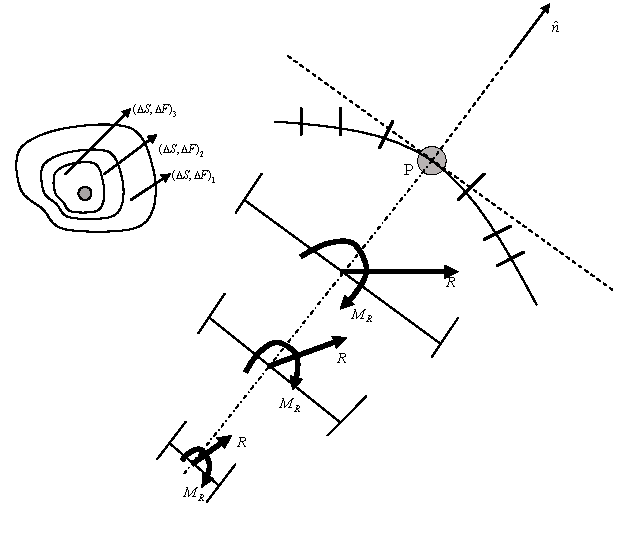
\includegraphics[width=4.0 in]{Cauchy1st.pdf}
	\caption{Vector de tracciones en un punto del medio continuo $P$.}
	\label{Cauchy1st}
\end{figure}

Para cada elemento de área considerado, la fuerza $\vec R$ y momento ${\vec
M_R}$ resultantes forman un ángulo determinado con la dirección $\hat{n}$. El
postulado de Cauchy propone que si se realiza un proceso continuo de reducción
de los elementos de área $\Delta S$, las cantidades $\left| {\vec R}
\right|/\Delta S$ y $\left| {{{\vec M}_R}} \right|/\Delta S$   tienden a límites
definidos. En el primer caso la función resultante $\vec t$ se denominará el
{\bf vector de tracciones} o {\bf fuerzas por unidad de superficie} en el punto
$P$ , \cref{trac}, mientras que en el segundo la función resultante $\vec \mu $
se denominará el vector de {\bf tracciones de par} o {\bf momentos por unidad de
superficie} y el cual asumiremos como cero en el estado límite,
\cref{couple}\footnote{El asumir este límite como cero da origen a un modelo
clásico de la mecánica de los medios continuos. Podría ser perfectamente válido
asumir este límite como diferente de cero.}.

\begin{equation}
{\vec t^{(\hat n)}} \equiv \mathop {\lim }\limits_{\Delta S(\hat n) \to 0} \frac{{\Delta \vec F}}{{\Delta S(\hat n)}} = \frac{{d\vec F}}{{dS}}.
\label{trac}
\end{equation}

\begin{equation}
{\vec \mu ^{(\hat n)}} \equiv \mathop {\lim }\limits_{\Delta S(\hat n) \to 0} \frac{{\Delta \vec M}}{{\Delta S(\hat n)}} = 0.
\label{couple}
\end{equation}


Mediante el proceso de límite fue posible reducir la interacción a nivel de la
superficie a puntos (función continua). El vector de tracciones representa
entonces una descripción intensiva de la interacción por contacto directo entre
las regiones interna y externa. Esta interacción debe además satisfacer la
tercera ley de Newton o principio de acción y reacción.

Como consecuencia nos encontramos con que este vector de tracciones es igual (en
magnitud) y opuesto (en dirección) a la representación de la interacción sobre
la región externa. Esta condición se expresa mediante la relación de equilibrio
de la \cref{third} para el punto $P$, \cref{Newton3rd}, y el diagrama de cuerpo
libre de la \cref{dcl_ext}.

\begin{equation}
{\vec t^{({{\hat n}^ + })}} + {\vec t^{({{\hat n}^ - })}} = 0
\label{third}
\end{equation}

\begin{figure}[H]
\centering
	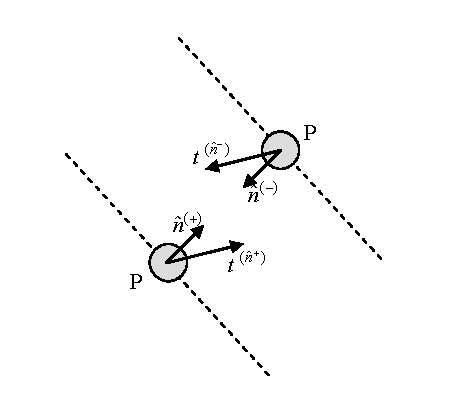
\includegraphics[width=2.8 in]{Newton3rd.pdf}
	\caption{Transmisión de tracciones a ambos lados de una superficie pasando por el punto $P$.}
	\label{Newton3rd}
\end{figure}

\subsection{Fuerzas por unidad de superficie sobre un plano con dirección normal $\hat{n}$}
Consideremos ahora el elemento diferencial de la \cref{TetraCauchy} el cual se ha
construido alrededor de un punto material $P$. En el elemento se han realizado
cortes a través de los 3 planos perpendiculares a los ejes cartesianos y con
vectores normales $-\hat{i}$, $-\hat{j}$ y $-\hat{k}$ y a través de un plano
inclinado con vector normal $\hat{n}=n_x \hat{i}+n_y \hat{j}+n_z \hat{k}$. Sobre
este plano también se traza un vector $\hat{\nu}=\nu_x \hat{i}+\nu_y
\hat{j}+\nu_z \hat{k}$ paralelo al plano. Los vectores de tracción sobre los
planos cartesianos están dados por ${{\vec t}^{( - \hat i)}}$ , ${{\vec t}^{( -
\hat j)}}$ y ${{\vec t}^{( - \hat k)}}$, mientras que el vector de tracciones
sobre el plano inclinado está dado por ${{\vec t}^{(n)}}$. Si se sabe que el
plano de corte tiene un vector de superficie $d\vec S = dS\hat n$, donde $dS$ es
el área de la sección superficial, se desea plantear las ecuaciones de equilibrio en las direcciones $\hat{n}$ y $\hat{\nu}$.

Para resolver el problema será necesario convertir los vectores de tracción
sobre cada una de las caras a vectores fuerza y posteriormente proyectar las
fuerzas resultantes en las direcciones $\hat{n}$ y $\hat{\nu}$. Denotando las
componentes escalares del vector ${{\vec t}^{(n)}}$ a lo largo de las
direcciones $\hat{n}$ y $\hat{\nu}$ como ${\sigma _{nn}}$ y ${\tau _{n\nu }}$
respectivamente, este puede escribirse como;

\begin{equation}
{{\vec t}^{(\hat n)}} = {\sigma _{nn}}\hat n + {\tau _{n\nu }}\hat \nu.
\label{incltract}
\end{equation}
%
\begin{figure}[H]
\centering
	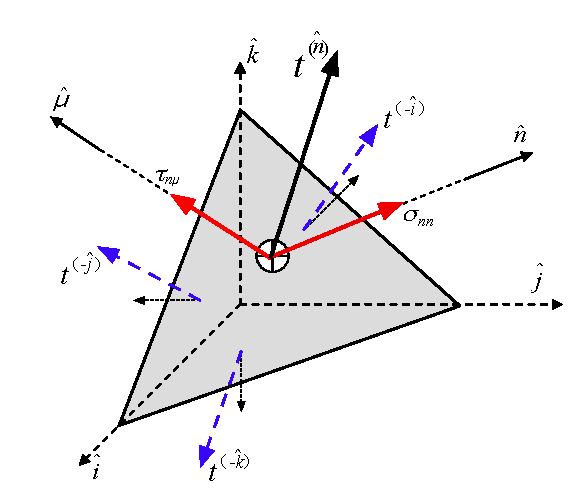
\includegraphics[width=3.5 in]{TetaCauchy.pdf}
	\caption{Elemento diferencial cortado con un plano de vector normal $\hat{n}$ tras lo cual se expone el vector de tracciones ${{\vec t}^{(n)}}$.}
	\label{TetraCauchy}
\end{figure}
%


Planteando primero $\sum {{F_n} = 0}$ se tiene;

\[{\sigma _{nn}}dS - [{{\vec t}^{( - \hat i)}} \cdot \hat n]d{S_x} - [{{\vec t}^{( - \hat j)}} \cdot \hat n]d{S_y} - [{{\vec t}^{( - \hat k)}} \cdot \hat n]d{S_z} = 0.\]


Ahora, expresando los vectores de tracción ${{\vec t}^{( - \hat i)}}$ , ${{\vec
t}^{(-\hat j)}}$ y ${{\vec t}^{( - \hat k)}}$ en términos de sus componentes
escalares en las direcciones $\hat{i}$, $\hat{j}$ y $\hat{k}$ es posible escribir la expresión anterior como:

\begin{align*}
{\sigma _{nn}}dS - ({\sigma _{xx}}{n_x} + {\tau _{xy}}{n_y} + {\tau _{xz}}{n_z})d{S_x} - ({\tau _{yx}}{n_x} + {\sigma _{yy}}{n_y}\\
+ {\tau _{yz}}{n_z})d{S_y} - ({\tau _{zx}}{n_x} + {\tau _{zy}}{n_y} + {\sigma _{zz}}{n_z})d{S_z}=0
\end{align*}

finalmente, escribiendo las áreas de los planos cartesianos $dS_x$, $dS_y$ y $dS_z$ en términos del área $dS$ del plano inclinado de acuerdo con:

\begin{align*}
d{S_x} = dS{n_x}\\
d{S_y} = dS{n_y}\\
d{S_z} = dS{n_z}
\end{align*}

se tiene que la fuerza por unidad de superficie en la dirección normal al plano de corte está dada por:

\begin{equation}
\begin{aligned}
{\sigma _{nn}} = {\sigma _{xx}}n_x^2 + {\tau _{xy}}{n_x}{n_y} + {\tau _{xz}}{n_x}{n_z} + {\tau _{yx}}{n_x}{n_y}\\
 + {\sigma _{yy}}n_y^2 + {\tau _{yz}}{n_z}{n_y} + {\tau _{zx}}{n_x}{n_z} + {\tau _{zy}}{n_y}{n_z} + {\sigma _{zz}}n_z^2.
\end{aligned}
\label{sigmann}
\end{equation}

Procediendo de manera similar planteamos $\sum {{F_\nu} = 0}$ como;

\[{\tau _{n\nu}}dS - [{{\vec t}^{( - \hat i)}} \cdot \hat \nu]d{S_x} - [{{\vec t}^{( - \hat j)}} \cdot \hat \nu]d{S_y} - [{{\vec t}^{( - \hat k)}} \cdot \hat \nu]d{S_z} = 0.\]


y expresando nuevamente los vectores de tracción en términos de sus componentes escalares obtenemos;
\begin{align*}
{\tau _{n\nu}}dS - ({\sigma _{xx}}{\nu_x} + {\tau _{xy}}{\nu_y} + {\tau _{xz}}{\nu_z})d{S_x} - ({\tau _{yx}}{\nu_x} + {\sigma _{yy}}{\nu_y}\\
+ {\tau _{yz}}{\nu_z})d{S_y} - ({\tau _{zx}}{\nu_x} + {\tau _{zy}}{\nu_y} + {\sigma _{zz}}{\nu_z})d{S_z}=0.
\end{align*}

Luego de usar nuevamente las expresiones para las áreas de las caras asociadas a los planos cartesianos en términos del área del plano inclinado de acuerdo con:
\begin{align*}
d{S_x} = dS{n_x}\\
d{S_y} = dS{n_y}\\
d{S_z} = dS{n_z}
\end{align*}

se tiene que la fuerza por unidad de superficie en la dirección paralela al plano de corte está dada por:

\begin{equation}
\begin{aligned}
{\tau _{n\nu}} = {\sigma _{xx}}{\nu_x}{n_x} + {\tau _{xy}}{\nu_y}{n_x} + {\tau _{xz}}{\nu_z}{n_x} + {\tau _{yx}}{\nu_x}{n_y}\\
 + {\sigma _{yy}}{\nu_y}{n_y} + {\tau _{yz}}{\nu_z}{n_y} + {\tau _{zx}}{\nu_x}{n_z} + {\tau _{zy}}{\nu_y}{n_z} + {\sigma _{zz}}{\nu_z}{n_z}.
\end{aligned}
\label{taunu}
\end{equation}

\subsection{Tensor de tensiones}
De las \cref{sigmann} y \cref{taunu} es posible concluir que para determinar
completamente el vector de tracciones ${{\vec t}^{(n)}}$ en el punto material
$P$ sobre una superficie con dirección normal $\hat{n}$ es necesario conocer los
vectores de tracción ${{\vec t}^{( - \hat i)}}$ , ${{\vec t}^{( - \hat j)}}$ y
${{\vec t}^{( - \hat k)}}$ asociados con 3 direcciones 
perpendiculares.\footnote{Es posible demostrar que en realidad basta con conocer los 3 vectores de tracción sobre planos asociados con 3 direcciones no co-lineales y no necesariamente ortogonales. Sin embargo por conveniencia se eligen las 3 direcciones cartesianas.}

Estos 3 vectores de tracción (o equivalentemente sus respectivas componentes
escalares) forman una cantidad tensorial (tensor de orden 2) denominada el
tensor de tensiones. Estos permiten definir de manera completa el estado de fuerzas
por unidad de superficie en asocio con cualquier dirección de un punto material del medio
continuo. Es común almacenar o representar este tensor en una matriz de $3
\times 3$ en la cual cada vector fila almacena las componentes escalares de los vectores de tracción.

\[\left[ {\begin{array}{*{20}{c}}
{{\sigma _{xx}}}&{{\tau _{xy}}}&{{\tau _{xz}}}\\
{{\tau _{yx}}}&{{\sigma _{yy}}}&{{\tau _{yz}}}\\
{{\tau _{zx}}}&{{\tau _{zy}}}&{{\sigma _{zz}}}
\end{array}} \right]\]

La \cref{stress} muestra estos vectores y sus componentes escalares. En dicha
figura y en la representación matricial del tensor de tensiones los índices $i$
y $j$ en un término típico $\sigma_{ij}$ hacen referencia al plano sobre el que
está aplicado el vector de tracciones y a la dirección sobre la cual se está proyectando el mismo.

\begin{figure}[H]
\centering
	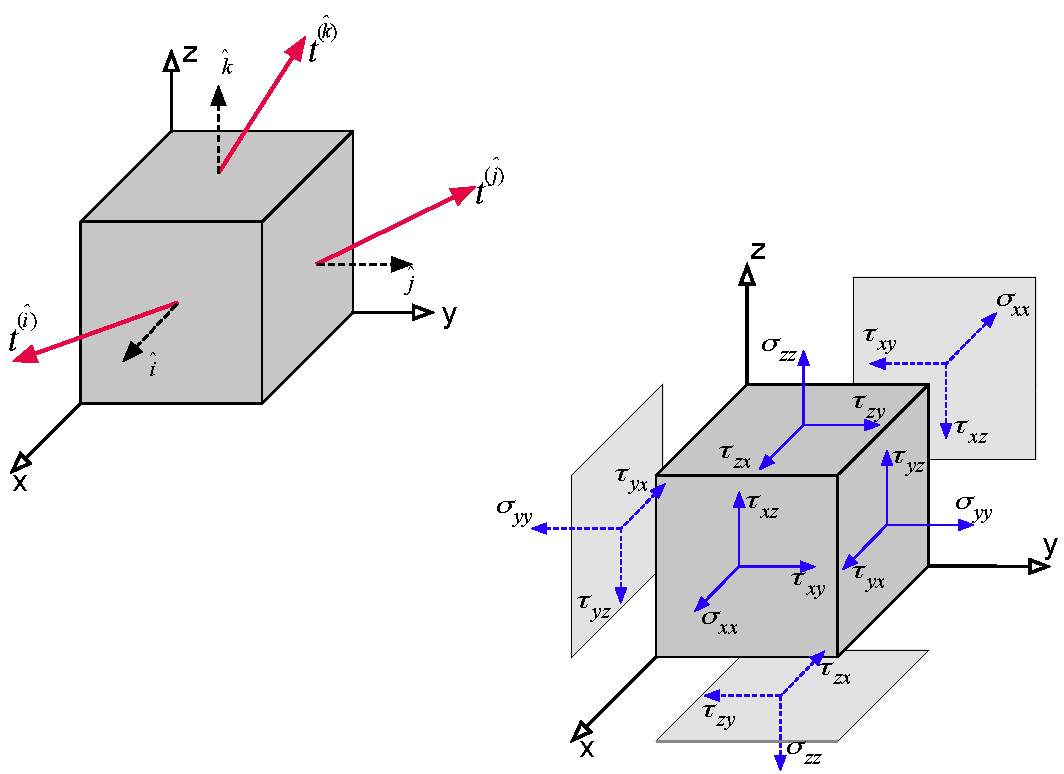
\includegraphics[width=5.0 in]{stress.pdf}
	\caption{Vectores de tracción actuando sobre los planos de un elemento diferencia en un sistema de referencia Cartesiano.}
	\label{stress}
\end{figure}

En esta representación también se han utilizado los simbolos $\sigma$ y $\tau$
para diferenciar las componentes normales (almacenadas en la diagonal de la matriz) y paralelas al plano (almacenadas por fuera de la diagonal de la matriz). Por
ejemplo la componente $\tau_{xy}$ hace referencia a la proyección en la
dirección $\hat{j}$ (índice y) del vector de tracciones asociado al plano con
normal $\hat{i}$ (índice x). Similarmente, la componente $\tau_{zx}$ hace
referencia a la proyección en la dirección $\hat{i}$ (índice x) del vector de
tracciones asociado al plano con normal $\hat{k}$ (índice z).

\subsubsection{Cálculo del vector de tracciones sobre un plano con vector normal
$\hat{n}$ (Formula de Cauchy).}
En la sección anterior se derivaron las \cref{sigmann} y
\cref{taunu} las cuales permitían calcular las componentes
$\sigma_{nn}$ y $\tau_{n\nu}$ que definían el vector de tracciones ${{\vec t}^{(n)}}$ en el plano inclinado con vector normal $\hat{n}$, mediante las 9 componentes escalares del tensor de tensiones (o esfuerzos). Nótese que estas componentes permiten expresar el vector ${{\vec t}^{(n)}}$ en el sistema de referencia $\hat{n}-\hat{\nu}$ de acuerdo con:


\[ {{\vec t}^{(\hat n)}} = {\sigma _{nn}}\hat n + {\tau _{n\nu }}\hat \nu. \]

Aunque desde el punto de vista físico las componentes  $\sigma_{nn}$ y $\tau_{n\nu}$ son bastante útiles toda vez que dan cuenta de lo que experimenta el medio a lo largo del plano en térmios de tensiones normales y paralelas a este, en ocasiones resulta útil o inclusive necesario el determinar directamente el vector ${{\vec t}^{(n)}}$ en el sistema de referencia $x-y-z$ en el cual se conoce el tensor de tensiones $\sigma_{ij}$. Este cálculo corresponde simplemente a la proyección en la dirección $\hat{n}$ de cada uno de los vectores  ${{\vec t}^{(\hat i)}}$ , ${{\vec t}^{(\hat j)}}$ y ${{\vec t}^{(\hat k)}}$ que definen el estado de tensiones en el punto $P$ como se ilustra a continuación.

Primero escribimos el vector ${{\vec t}^{(n)}}$ en términos de sus componentes escalares $t_x^{(\hat n)}$, $t_y^{(\hat n)}$ y $t_z^{(\hat n)}$  como:


\[{{\vec t}^{(\hat n)}} = t_x^{(\hat n)}\hat i + t_y^{(\hat n)}\hat j + t_z^{(\hat n)}\hat k.\]

Estas componentes se obtienen tras plantear y resolver las ecuaciones de equilibrio del elemento mostrado en la \cref{TetraCauchy} en las direcciones $\hat{i}$, $\hat{j}$  y $\hat{k}$ respectivamente. Las ecuaciones resultantes pueden escribirse de la forma:


\begin{align*}
t_x^{(\hat n)} = {{\vec t}^{(\hat i)}} \cdot \hat n\\
t_y^{(\hat n)} = {{\vec t}^{(\hat j)}} \cdot \hat n\\
t_z^{(\hat n)} = {{\vec t}^{(\hat k)}} \cdot \hat n
\end{align*}

o en la siguiente ecuación matricial:

\begin{equation}
\left\{ {\begin{array}{*{20}{c}}
{t_x^{(\hat n)}}\\
{t_y^{(\hat n)}}\\
{t_z^{(\hat n)}}
\end{array}} \right\} = \left[ {\begin{array}{*{20}{c}}
{{\sigma _{xx}}}&{{\tau _{xy}}}&{{\tau _{xz}}}\\
{{\tau _{yx}}}&{{\sigma _{yy}}}&{{\tau _{yz}}}\\
{{\tau _{zx}}}&{{\tau _{zy}}}&{{\sigma _{zz}}}
\end{array}} \right]\left\{ {\begin{array}{*{20}{c}}
{{n_x}}\\
{{n_y}}\\
{{n_z}}
\end{array}} \right\}.
\label{CauchyFormula}
\end{equation}

La \cref{CauchyFormula} correspondiente al producto entre el tensor de tensiones y el vector normal a una plano (o superficie de corte) se conoce como la fórmula de Cauchy. Matemáticamente ésta no es otra cosa que la proyección del tensor $\sigma_{ij}$ a lo largo de la dirección $\hat{n}$. De manera condensada la \cref{CauchyFormula} se puede escribir como:

\begin{equation}
\left\{ {{t^{(n)}}} \right\} = \left[ \sigma  \right]\left\{ n \right\}
\label{CauchyFormulaC}
\end{equation}

\subsubsection*{Ejemplo 1: Tracciones sobre un plano arbitrario a partir de $\sigma_{ij}$}
El estado de tensiones sobre un punto material $P$ de un medio continuo está
dado por $\sigma_{ij}$. Determinar el vector de tracciones sobre un plano $T$
definido por los puntos $A$, $B$ y $C$. Adicionalmente determinar las
componentes de la tensión en la dirección normal y paralela al plano.
\subsubsection*{Solución}
Primero necesitamos determinar la ecuación del plano definido por los puntos $A$, $B$ y $C$ y la dirección del vector normal. Recodando que la ecuación del plano esta dada por

\[ax+by+cz=d\]

donde los coeficientes $a$, $b$ y $c$ son las componentes del vector normal $\hat{n}$. Se tiene entonces que:

\[\hat n = \frac{{{{\vec r}_{AC}} \times {{\vec r}_{AB}}}}{{\left\| {{{\vec r}_{AC}} \times {{\vec r}_{AB}}} \right\|}}\]

luego:

\begin{align*}
&a \equiv {n_x}\\
&b \equiv {n_y}\\
&c \equiv {n_z}
\end{align*}

mientras que $d=a x_A+b y_A+c z_A$. Ahora es posible determinar el vector de tracciones sobre una superficie con vector normal $\hat{n}$ usando la \cref{CauchyFormula}:


\[
\left\{ {\begin{array}{*{20}{c}}
{t_x^{(\hat n)}}\\
{t_y^{(\hat n)}}\\
{t_z^{(\hat n)}}
\end{array}} \right\} = \left[ {\begin{array}{*{20}{c}}
{{\sigma _{xx}}}&{{\tau _{xy}}}&{{\tau _{xz}}}\\
{{\tau _{yx}}}&{{\sigma _{yy}}}&{{\tau _{yz}}}\\
{{\tau _{zx}}}&{{\tau _{zy}}}&{{\sigma _{zz}}}
\end{array}} \right]\left\{ {\begin{array}{*{20}{c}}
{{n_x}}\\
{{n_y}}\\
{{n_z}}
\end{array}} \right\}.
\]

Para determinar las componentes normal y paralela se proyecta el vector ${{\vec t}^{(\hat n)}}$ a lo largo de $\hat{n}$. Si se denotan las componentes de ${{\vec t}^{(\hat n)}}$ por $t_x^{(\hat n)}$, $t_y^{(\hat n)}$  y $t_z^{(\hat n)}$  se tiene que:

\[{\sigma _{nn}} = {{\vec t}^{(\hat n)}} \cdot \hat n \equiv t_x^{(\hat n)}{n_x} + t_y^{(\hat n)}{n_y} + t_z^{(\hat n)}{n_z}\]

mientras que la tensión paralela al plano de corte se determina como:

\[\tau _{n\nu }^2 = {{\vec t}^{(\hat n)}} \cdot {{\vec t}^{(\hat n)}} - \sigma _{nn}^2\]


\subsection{Transformación por rotación. Caso general}

Al igual que en el caso vectorial, en varias aplicaciones será conveniente conocer la descripción del tensor de tensiones bajo la rotación de su
sistema de referencia, o más interesante aún, deseamos saber como varían las tensiones en las diferentes direcciones de un punto material del medio continuo. Este problema corresponde al problema de {\bf transformación bajo rotación} o la determinación de las componentes del tensor de tensiones en un sistema de referencia primado $x'-y'-z'$ a partir de las componentes en un sistema de referencia no primado $x-y-z$, ver \cref{rotation}. 


\begin{figure}[H]
\centering
	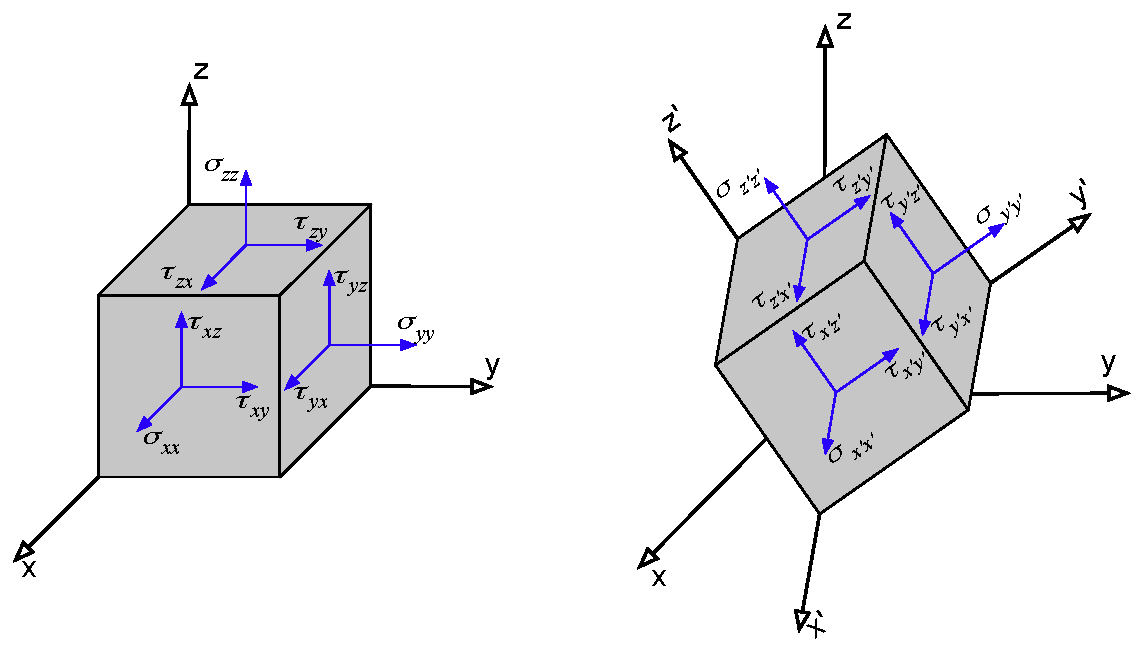
\includegraphics[width=5.0 in]{rotation.pdf}
	\caption{Representación de tensor de tensiones en un sistema $x-y-z$ y en un sistema alternativo $x'-y'-z'$ rotado con respecto al primero.}
	\label{rotation}
\end{figure}

En la figura se hace la descripción esquemática del tensor en el sistema primado y no primado respectivamente. En la sección anterior se resolvió el problema de la determinación del vector de tracciones en asocio con una dirección normal $\hat{n}$ (ver \cref{CauchyFormula}). Para resolver el problema de transformación bajo rotación basta con reconocer las direcciones $\hat{i'}$, $\hat{j'}$ y $\hat{k'}$  del nuevo sistema de referencia como vectores normales a lo largo de los cuales se desea determinar los vectores de tracciones ${\vec t^{(i')}}$, ${\vec t^{(j')}}$ y ${\vec t^{(k')}}$. En la \cref{roteje} se presentan en línea púrpura las direcciones asociadas con el sistema de referencia $x-y-z$, mientras que en línea negra se presentan las direcciones asociadas con el sistema de referencia primado $x'-y'-z'$. Denotaremos por $\sigma$ al tensor de tensiones en el primer sistema de referencia y por $\sigma'$ el del segundo. 

\begin{figure}[H]
\centering
	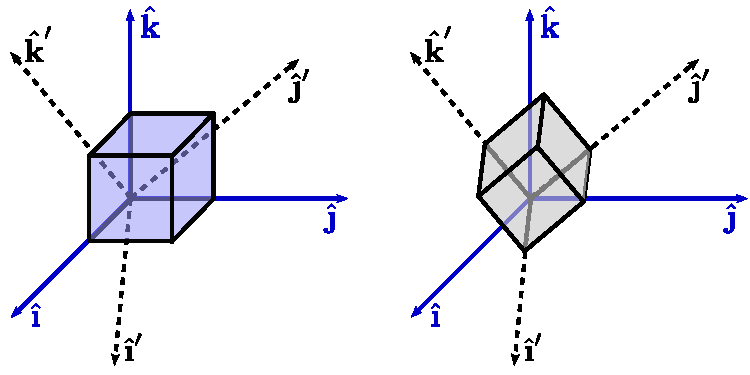
\includegraphics[width=2.8 in]{rota_ejes.pdf}
	\caption{Representación de tensor de tensiones en sistema $x-y-z$ y $x'-y'-z'$.}
	\label{roteje}
\end{figure}


Utilizando la \cref{CauchyFormula}, o equivalentemente la \cref{CauchyFormulaC} determinemos el vector de tracciones en caras
con vectores normales $\hat{i'}$, $\hat{j'}$ y $\hat{k'}$ de acuerdo con:
%

\begin{equation}
\begin{aligned}
&\left\{ {{t^{(i')}}} \right\} = \left[ \sigma  \right]\left\{ i' \right\} \\
&\left\{ {{t^{(j')}}} \right\} = \left[ \sigma  \right]\left\{ j' \right\} \\
&\left\{ {{t^{(k')}}} \right\} = \left[ \sigma  \right]\left\{ k' \right\}
\end{aligned}
\label{proy1}
\end{equation}
%
Ahora, estos vectores deben ser expresados en términos de componentes escalares en el sistema de referencia $x'-y'-z'$ para lo cual proyectamos cada uno de ellos a lo largo de las direcciones $\hat{i'}$, $\hat{j'}$ y $\hat{k'}$ como sigue;

\begin{equation}
\begin{aligned}
&{{\vec t}^{(i')}} = [{{\vec t}^{(i')}} \cdot \hat i']\hat i' + [{{\vec t}^{(i')}} \cdot \hat j']\hat j' + [{{\vec t}^{(i')}} \cdot \hat k']\hat k' \\
&{{\vec t}^{(j')}} = [{{\vec t}^{(j')}} \cdot \hat i']\hat i' + [{{\vec t}^{(j')}} \cdot \hat j']\hat j' + [{{\vec t}^{(j')}} \cdot \hat k']\hat k' \\
&{{\vec t}^{(k')}} = [{{\vec t}^{(k')}} \cdot \hat i']\hat i' + [{{\vec t}^{(k')}} \cdot \hat j']\hat j' + [{{\vec t}^{(k')}} \cdot \hat k']\hat k'
\end{aligned}
\label{proy2}
\end{equation}

Estas expresiones equivalen a:
%
\begin{align*}
& {{\vec t}^{(i')}} = {\sigma _{x'x'}}\hat i' + {\tau _{x'y'}}\hat j' + {\tau _{x'z'}}\hat k' \\
& {{\vec t}^{(j')}} = {\tau _{y'x'}}\hat i' + {\sigma _{y'y'}}\hat j' + {\tau _{y'z'}}\hat k' \\
&{{\vec t}^{(k')}} = {\tau _{z'x'}}\hat i' + {\tau _{z'y'}}\hat j' + {\sigma _{z'z'}}\hat k'.
\end{align*} \\

%
Finalmente si escribimos los vectores $\hat{i'}$, $\hat{j'}$ y $\hat{k'}$ en el sistema de referencia $x-y-z$ en términos de sus cosenos directores como:

\begin{equation}
\begin{aligned}
&\hat i' = {C_{x'x}}\hat i + {C_{x'y}}\hat j + {C_{x'z}}\hat k \\
&\hat j' = {C_{y'x}}\hat i + {C_{y'y}}\hat j + {C_{y'z}}\hat k \\
&\hat k' = {C_{z'x}}\hat i + {C_{z'y}}\hat j + {C_{z'z}}\hat k
\end{aligned}
\label{cosdir}
\end{equation}

Substituyendo las \cref{proy1} y \cref{cosdir} en la \cref{proy2} se tiene:

%
\begin{align}
[\sigma'] = [C] [\sigma] {[C]^T}
\label{rotacion}
\end{align}
%
donde $[C]$,  que es conocida como la matriz de cosenos que relacionan los dos
sistemas y está dada por: \\
\[
[C]
= 
\begin{bmatrix}
    C_{x'x} & C_{x'y} & C_{x'z} \\
    C_{y'x} & C_{y'y} & C_{y'z} \\
    C_{z'x} & C_{z'y} & C_{z'z}
\end{bmatrix}
\]

\subsection{Transformación por rotación 2D. Círculo de Mohr}
%
En muchas aplicaciones prácticas los problemas de tensiones pueden ser estudiados mediante un análisis en dos dimensiones. Cuando éste es el caso la transformación por rotación puede ser desarrollada a partir de una herramienta gráfica conocida como el círculo de Mohr.  En lo que sigue se deducen las expresiones para pasar de un tensor con representación en un sistema $x-y$ a su respresentación en un sistema primado $x'-y'$. En la \cref{rota2D} se muestra la descripción esquemática del tensor en el sistema primado y no primado respectivamente. 

\begin{figure}[H]
\centering
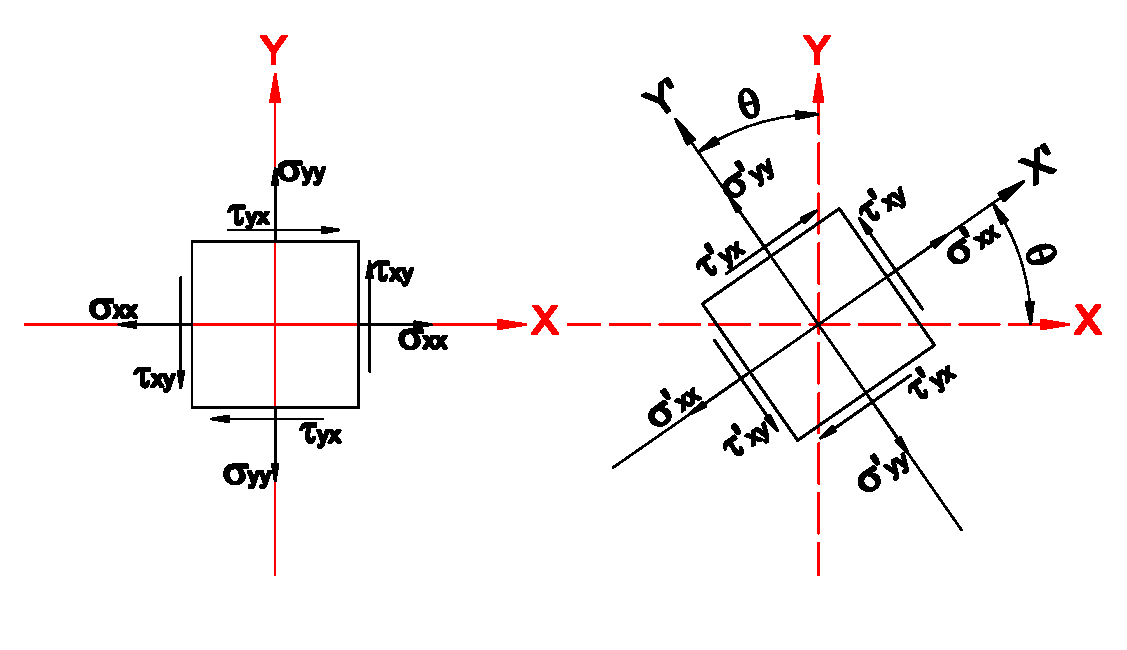
\includegraphics[scale=.7]{Rotacion_tensor.pdf}
\caption{Izquierda: Tensor $[\sigma]$ en el sistema de referencia $x-y$, Derecha: Tensor $[\sigma ']$ en el sistema de referencia $x'-y'$. El sistema de referencia $x'-y'$ se encuentra rotado un ángulo $\theta$ respecto a $x-y$.} 
\label{rota2D}
\end{figure} 
%
Desarrollando de la forma expandida la  ley de transformación por rotación presentada en \cref{rotacion}, para el caso 2D se tiene: \\
%
\begin{equation}
\left[ 
\begin{array}{ccc}
\sigma '_{xx} & \tau '_{xy} \\
\tau '_{xy} & \sigma '_{yy}
\end{array}
\right] =
\left[ 
\begin{array}{ccc}
C_\theta & S_\theta \\
-S_\theta & C_\theta
\end{array}
\right]
\left[ 
\begin{array}{ccc}
\sigma_{xx} & \tau_{xy} \\
\tau_{xy} & \sigma_{yy}
\end{array}
\right]
\left[ 
\begin{array}{ccc}
C_\theta & -S_\theta \\
S_\theta & C_\theta
\end{array}
\right]
\label{trans2d}
\end{equation}

Desarrollando la multiplicación matricial y escribiendo las tres expresiones que definen los tres escalares $\sigma ' _{xx}$, $\sigma ' _{yy}$ y $\tau ' _{xy}$:\\

\begin{equation}
\begin{aligned}
&\sigma ' _{xx} = \sigma _{xx} C^2 _\theta + \sigma _{yy} S^2 _\theta + 2 \tau _{xy} S _\theta C _\theta \\
&\sigma ' _{yy} = \sigma _{xx} S^2 _\theta + \sigma _{yy} C^2 _\theta - 2 \tau _{xy} S _\theta C _\theta \\
&\tau ' _{xy} = (\sigma _{yy} - \sigma _{xx}) S_\theta C _\theta +  \tau _{xy} (C^2 _\theta - S^2 _\theta) \\
\end{aligned}
\label{trans}
\end{equation}
%

Sumando la primera y la  segunda en la expresion anterior se tiene:

\begin{equation}
	\sigma ' _{xx} + \sigma ' _{yy} =   \sigma _{xx} +  \sigma _{yy}
	\label{inva}
\end{equation}
%
La  \cref{inva} muestra que la suma de las componentes normales (elementos sobre la diagonal) es invariante (no cambia) bajo la rotación del sistema de referencia. Eliminando $\sigma ' _{yy}$, se tiene:\\
%
\begin{equation}
	\sigma ' _{xx} -(\sigma _{xx} + \sigma _{yy}) = -(\sigma _{xx} S^2 _\theta + \sigma _{yy} C^2 _\theta - 2 \tau _{xy} S _\theta C_\theta). \\
\label{sigypyp}
\end{equation}
%
Utilizando las relaciones trigonométricas:\\
\\
	$sen ^2 \theta = \frac{1}{2} \left( 1 - cos \left( 2 \theta \right) \right)$\\\\
	$cos ^2 \theta = \frac{1}{2} \left( 1 + cos \left( 2 \theta \right) \right)$\\\\
	$ cos ^2 \theta -sen ^2 \theta =  cos \left( 2 \theta \right)$\\\\
	$sen \theta cos  \theta = \frac{1}{2} sen \left( 2 \theta \right)$ \\\\
%
la \cref{sigypyp} se puede reescribir como: \\

\begin{equation*}
	\sigma ' _{xx} -(\sigma _{xx} + \sigma _{yy}) = -\left[ \sigma _{xx} \frac{1-C_{2\theta}}{2} + \sigma _{yy} \frac{1+ C _{2\theta}}{2} - \tau _{xy} S_{2\theta} \right] \\
\end{equation*} \\\\

o agrupando términos: 
%
\begin{equation}
	\sigma ' _{xx} -\frac{\sigma _{xx} + \sigma _{yy}}{2} = \frac{\sigma_{xx} - \sigma _{yy}}{2} C_{2\theta} + \tau _{xy} S_{2\theta} 
\label{final1}
\end{equation}
\\
%
Reemplazando las identidades la tercer expresión de la \cref{trans2d} quedaría:\\
%
\begin{equation}
	\tau ' _{xy} = - \frac{\sigma _{xx} - \sigma _{yy}}{2} S_{2\theta} + \tau _{xy} C_{2\theta}
\label{final2}
\end{equation}
\\
%
Para terminar se suman los cuadrados de las \cref {final1}  y \cref {final2}
%
\begin{equation}
	\left[ \sigma ' _{xx} - \frac{\sigma _{xx} + \sigma _{yy} }{2} \right] ^2 + \left(\tau ' _{xy} \right)  ^2 =  \left( \frac{\sigma _{xx} - \sigma _{yy} }{2} \right) ^2 + \tau ^2 _{xy}
	\label{cir1}
\end{equation}
\\
Comparando la \cref{cir1} con la ecuación de un círculo, $r^2 = x^2 + y^2$, se puede concluir que ésta representa la ecuación de un círculo con radio $R$ y centro $C$  en el sistema de referencia $\sigma - \tau$.\\
%}
\begin{align}
	R ^ 2 = \left( \frac{\sigma _{xx} - \sigma _{yy}}{2} \right) ^2 + \tau ^2 _{xy} \\\\
	C = \left( \frac{\sigma _{xx} + \sigma _{yy}}{2},0 \right)
\end{align}
%
%

Reescribiendo la \cref{cir1} se tiene una ecuación describe todos los vectores de tracción asociados con las infinitas direcciones del espacio para un tensor dado de acuerdo con: \\
%
\begin{equation}
	\left(\sigma '_{xx}- C \right) ^2 + \left(\tau ' _{xy} \right) ^2 = R^2
\end{equation}
%
Las componentes del tensor en el espacio $\sigma$ vs $\tau $  corresponden a 2 puntos $A$  y $B$  dados por;\\
%
\begin{equation}
	\begin{array}{ccc}
	A=(\sigma_{xx}, -\tau _{xy}) \\
	B=(\sigma_{yy}, +\tau _{xy})
	\end{array}
	\label{puntos}
\end{equation}
%
El punto $A$  corresponde a la componente vectorial del tensor asociada con la dirección $\hat{i}$  mientras que el punto  $B$ corresponde a la componente vectorial del tensor asociada con la dirección $\hat{j}$ .  Nótese que en la \cref{puntos} el signo $(-)$  que antecede a la componente $\tau_{xy}$  del punto  $A$ es artificial.  Esto equivale a distorsionar la componente vectorial asociada con la dirección $\hat{i}$.  En la \cref{circulo} se representan los puntos $A$ y $B$ sobre el círculo. En este caso se asume que $\sigma_{yy} > \sigma_{xx}$ y $\tau_{xy} > 0$.\\
%
\begin{figure}[H]
\centering
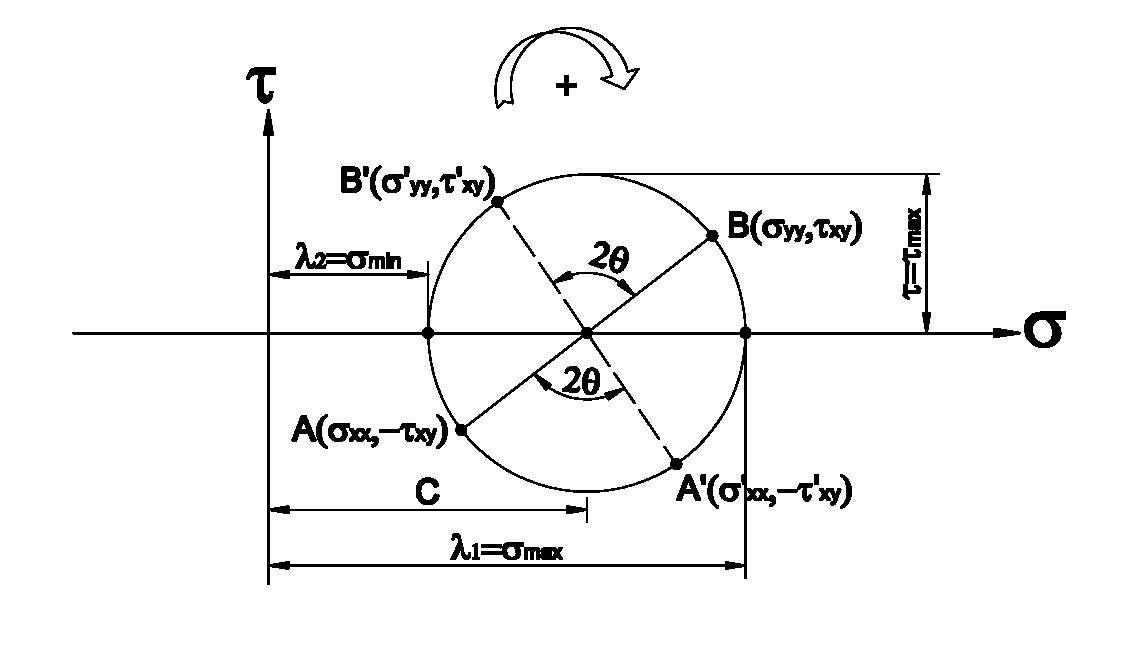
\includegraphics[scale=.7]{Circulo.pdf}
\caption{Círculo de Mohr para para $\sigma_{yy} > \sigma_{xx}$ y $\tau_{xy} > 0$.}
\label{circulo}
\end{figure}

En conclusión, dado el tensor de tensiones $\sigma_{ij}$ en el sistema de referencia $x-y$ es posible trazar el círculo correspondente al estado de esfuerzos en el punto mataerial y a partir de este se pueden determinar sus componentes en cualquier otra dirección. Esta aparece en el círculo con una orientación $2\theta$ con respecto a la dirección original debido a la parametrización de las ecuaciones en la derivación misma de la ecuación del círculo. En consecuencia, un angulo de $\theta$ en el problema físico aparece como  $2\theta$ en el círculo de Mohr.

Un problema de especial interés, y facilmente soluble con el círculo de Mohr, es el de determinar las direcciones en las cuales se presentan las máximas y mínimas tensiones normales y paralelas. Estas aparecen en el círculo de la \cref{circulo} rotuladas como ${\lambda _1} = {\sigma _{\max }}$, ${\lambda _2} = {\sigma _{\min }}$ y $\tau  = {\tau _{\max }}.$

%
\subsubsection*{Ejemplo 2: Círculo de Mohr} 

La \cref{planosEjMohr} muestra dos estados de tensiones para el mismo punto de
un medio continuo. 
%
\begin{figure}[H]
	\centering
		\subfloat [Estado de tensión 1]{ 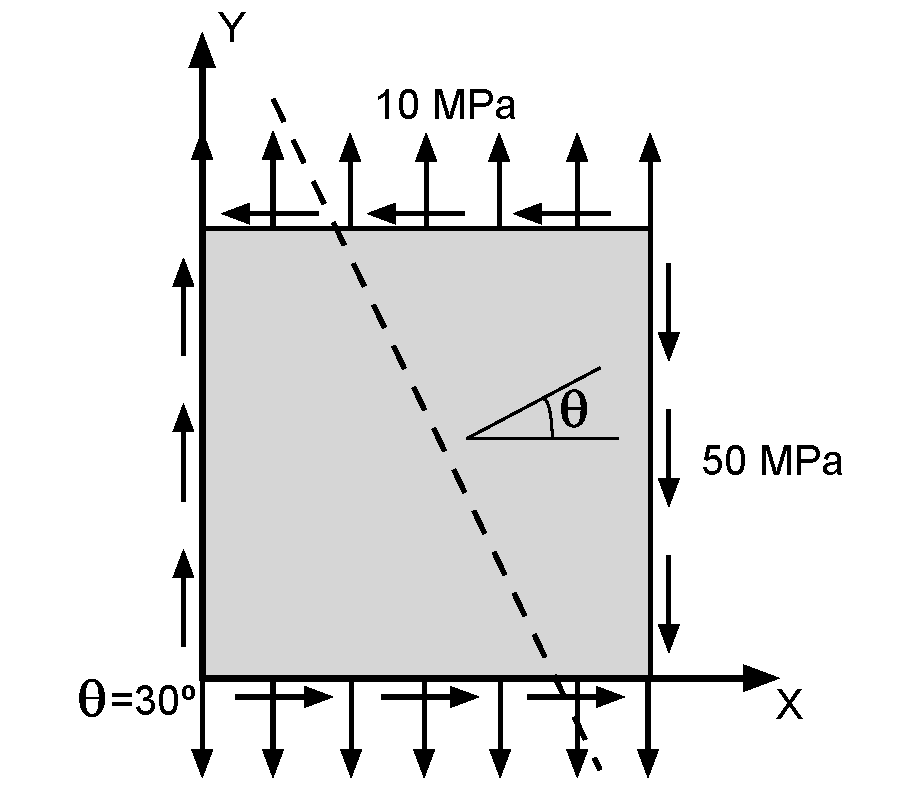
\includegraphics[width=2.8in]{Estado1.pdf}\label{Estado1EjMohr}}
		\hspace{0.5cm}
		\subfloat [Estado de tensión 2]{ 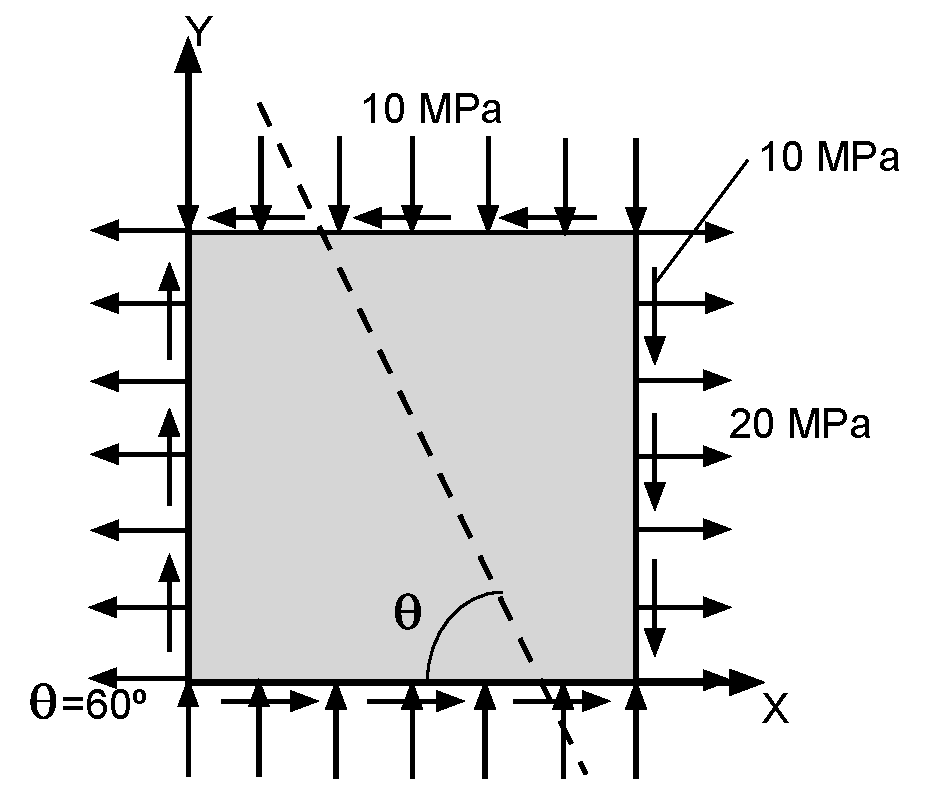
\includegraphics[width=2.5in]{Estado2.pdf}\label{Estado2EjMohr}}		
	\caption{Estado de tensiones en un punto. }
	\label{planosEjMohr}
\end{figure}
%
Para cada estado de carga mostrado en la  \cref{Estado1EjMohr} y en la  \cref{Estado2EjMohr}, respectivamente.
\begin{enumerate}
%
\item[•] Determinar los esfuerzos normales y cortantes sobre los planos mostrados con linea punteada. \\\\
%
\textbf{Solución:}\\\\
%
Inicialmente determinemos el tensor de tensiones para los estados $1$ y $2$
mostrados en la \cref{Estado1EjMohr} y la \cref{Estado2EjMohr} respectivamente.
%
\begin{equation*}
[\sigma_1] =
 	\begin{bmatrix}
     	0.0 & -50.0 & \\
     	-50.0 & 10.0 \\
 	\end{bmatrix}
 \hspace{1cm}
 [\sigma_2] =
 	\begin{bmatrix}
     	20.0 & -10.0 & \\
     	-10.0 & -10.0 \\
 	\end{bmatrix}
\end{equation*}
%
Aunque hay diversos caminos para llegar a una solución, para dar una mayor
ilustración del manejo del círculo de  Mohr haremos uso de esta herramienta
\footnote{Es buen ejercicio cotejar estos resultados haciendo uso del manejo
matricial de la transformación.}. En la  \cref{Tension1} y  en la \cref{Tension2}
se muestra el círculo de Mohr para ambos estados de tensiones. Dicho estado se indica mediante la línea $X-Y$.
%
\begin{figure}[H]
	\centering
		\subfloat [Estado de tensión 1]{ 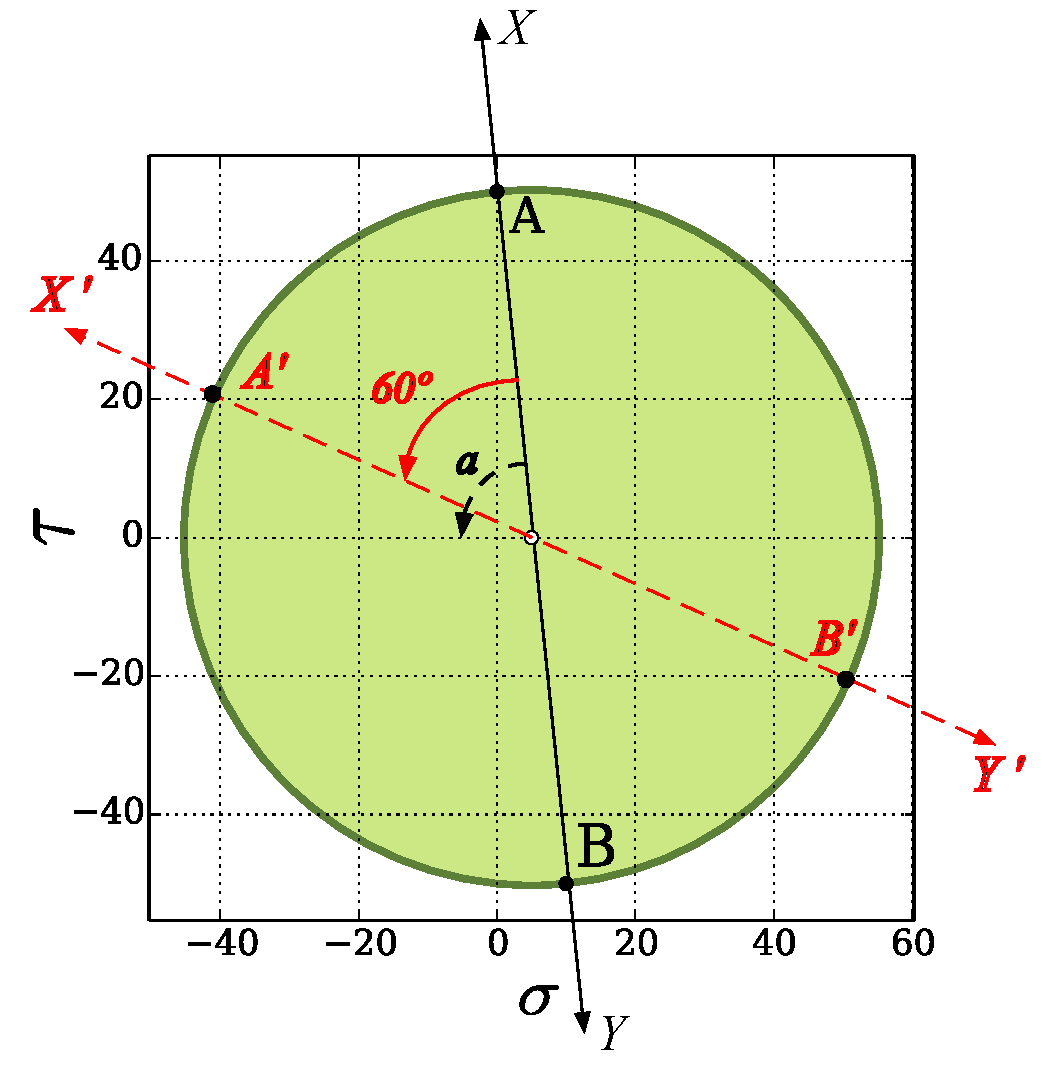
\includegraphics[width=2.5in]{Tensor1.pdf}\label{Tension1}}
		\hspace{0.5cm}
		\subfloat [Estado de tensión 2]{ 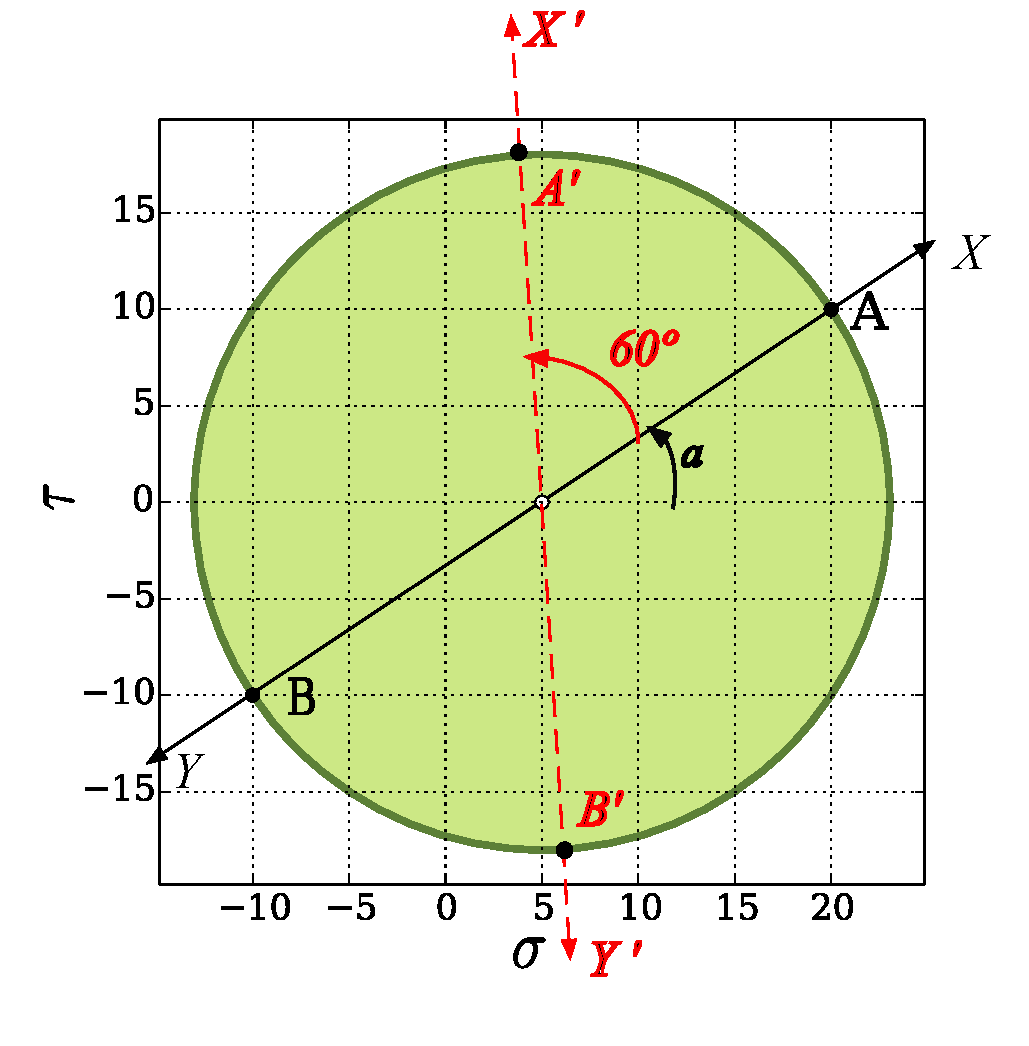
\includegraphics[width=2.5in]{Tensor2.pdf}\label{Tension2}}		
	\caption{Círculo de Mohr con tensor en sistema original $x-y$ y sistema rotado
	$x'-y'$ }
	\label{Tensiones}
\end{figure}
%
Para encontrar las tensiones normales y tangenciales solicitadas hacemos una
rotación de $60^{\circ}$ en el círculo de Mohr ($30^{\circ}$ en el problema
físico) en sentido contrario a las manecillas del reloj. Esta rotación se indica
en el círculo de Mohr de la \cref{Tensiones} mediante las líneas punteadas
color rojo $X'-Y'$ que unen los puntos $A'$ y $B'$. Si se lee la información
de los puntos $A'$ y $B'$ se obtienen los tensores en el sismema $x'-y'$. El
estado de tensiones en el sistema rotado sería entonces dado por:
%
\begin {equation}
\begin {aligned}
 &\tau'_{xy} = R  \sen (\beta) \\
 &\sigma'_{xx} = C - R  \cos(\beta) \\
 &\sigma'_{yy} = C + R  \cos(\beta) \\
\end {aligned}
\label{cicmohr1}
\end {equation}
%
Donde $R$ y $C$ son el radio  y el centro del círculo de Mohr
respectivamente.\\\\
%
Para el estado 1 $R = 50.25$, $C = 5.0$ y $\beta =\alpha - 60 ^{\circ}$. $\alpha
= \arctan\left(\dfrac{50}{5}\right)$ \\
%
Para el estado 2 $R = 18.03 $, $C = 5.0$ y $\beta =180^{\circ} - (\alpha +
60^{\circ})$. $\alpha = \arctan\left(\dfrac{10}{15}\right)$ \\\\
%
Los tensores en el sistema rotado serían: \\
 \begin{equation*}
[\sigma'_1] =
 	\begin{bmatrix}
     	-40.80 & -20.67 & \\
     	-20.67 & 50.80 \\
 	\end{bmatrix}
 \hspace{1cm}
 [\sigma'_2] =
 	\begin{bmatrix}
     	3.83 & -17.99 & \\
     	-17.99 & 6.16 \\
 	\end{bmatrix}
\end{equation*} \\
A partir de los tensores anteriores se concluye que las tensiones normal y tangencial
al plano solicitado son $\sigma=-40.80$ y  $\tau = -20.67$ para el estado $1$ y
$\sigma=3.83$ y  $\tau = -17.99$ para el estado $2$ respectivamente. En la
\cref{Cubo1} y en la \cref{Cubo2} se representa el cubo de tensiones para cada estado.
%

\begin{figure}[H]
	\centering
		\subfloat [Estado de tensión 1]{ 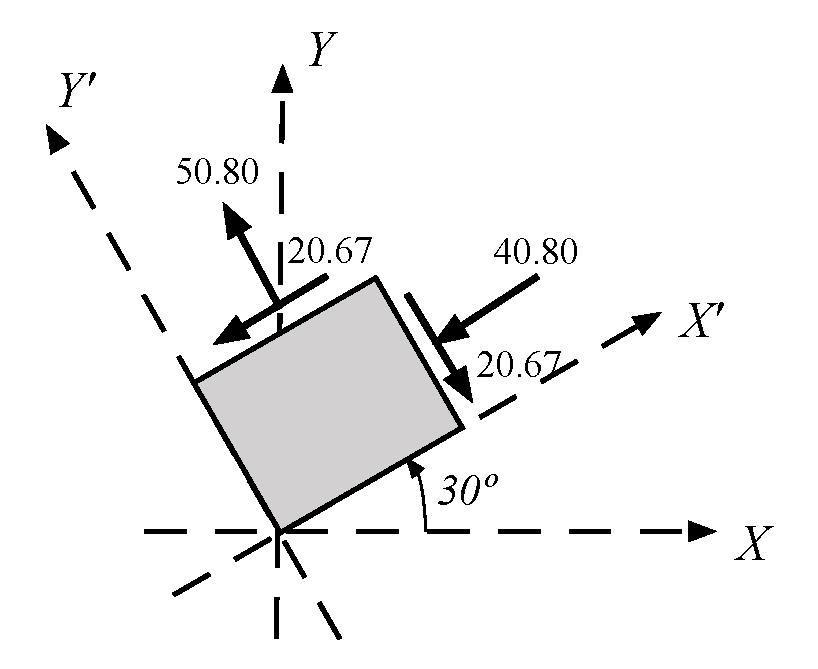
\includegraphics[width=2.5in]{Cubo1.pdf}\label{Cubo1}}
		\hspace{0.5cm}
		\subfloat [Estado de tensión 2]{ 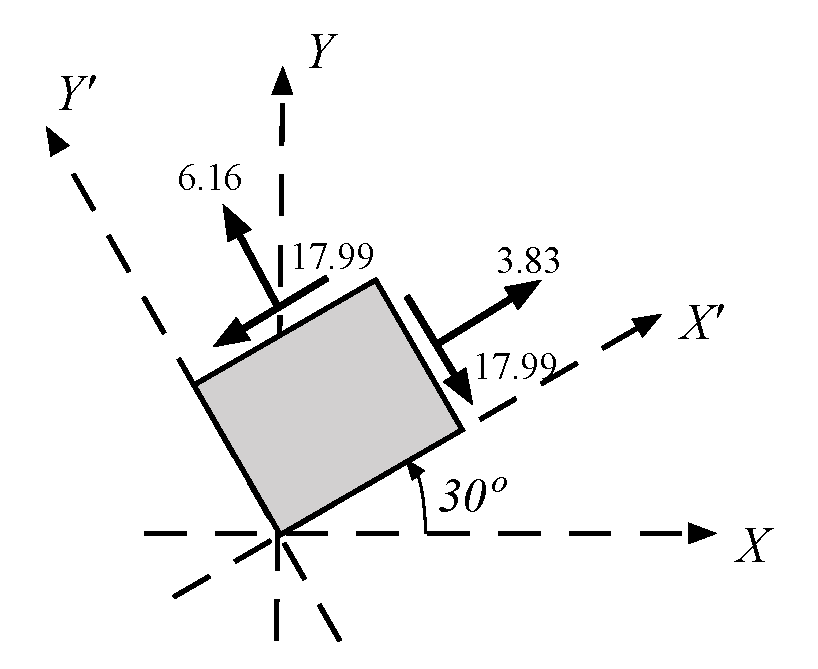
\includegraphics[width=2.5in]{Cubo2.pdf}\label{Cubo2}}		
	\caption{Cubo de Tensiones en sistema rotado $x'-y'$ }
	\label{Cubos}
\end{figure}

\item[•] Para cada uno de los estados de tensiones mostrados determinar los valores
propios y las direcciones principales. \\\\
%
\textbf{Solución:}\\\\
%
Los valores principales no son otra cosa que los valores máximos axiales
(normales) a los cuales está sometido el punto. Este estado se logra
precisamente cuando el valor de las tensiones tangenciales es nulo. En la
 \cref{Tens1Prin} y en la  \cref{Tens2Prin} se muestra en el círculo de Mohr, el
sistema original $x-y$ y el sistema principal $x_p - y_p$, mientras que en la \cref{Cubo1Prin} y en la  \cref{Cubo2Prin} se muestra el cubo de tensiones para
el estado principal.


\begin{figure}[H]
	\centering
		\subfloat [Estado de tensión 1]{ 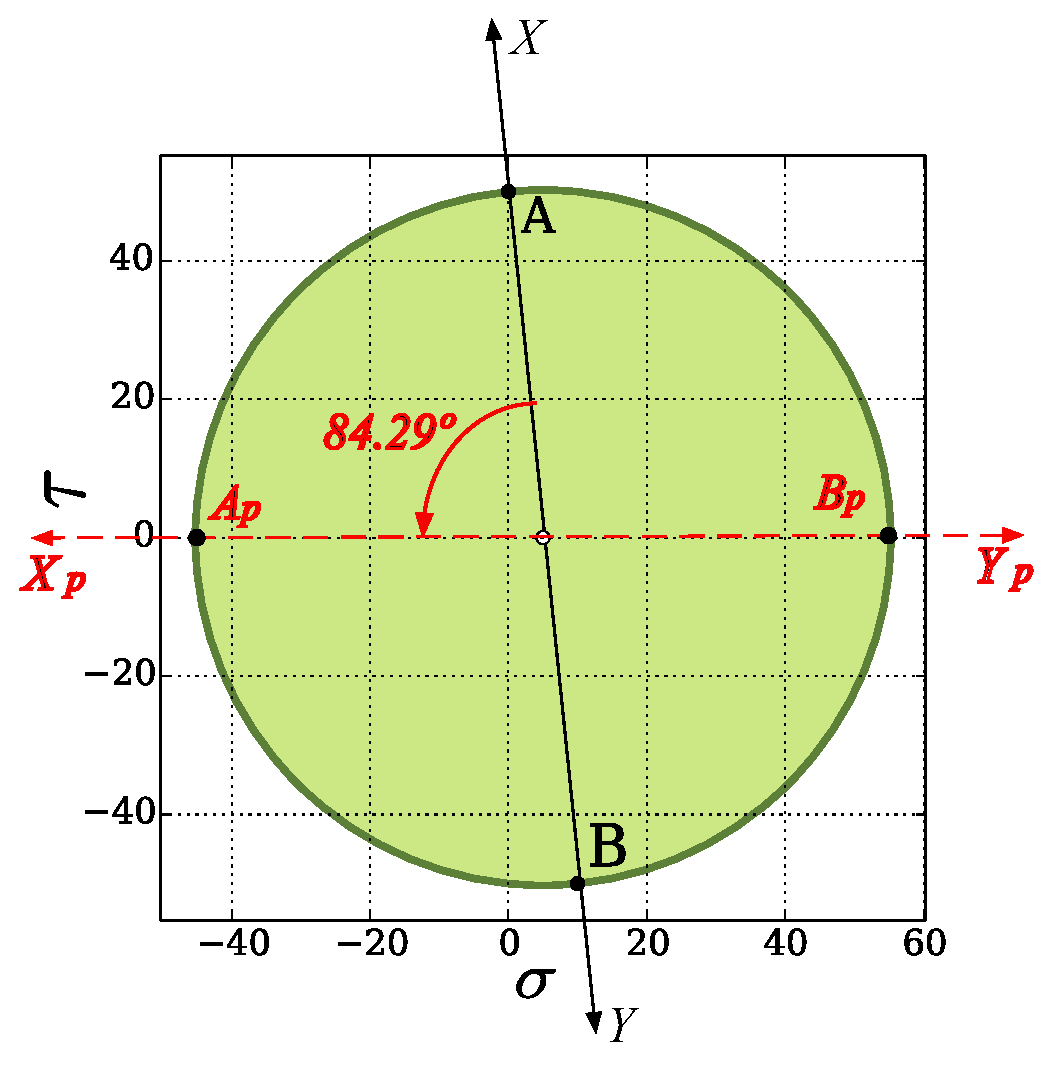
\includegraphics[width=2.5in]{Tens1Prin.pdf}\label{Tens1Prin}}
		\hspace{0.5cm}
		\subfloat [Estado de tensión 2]{ 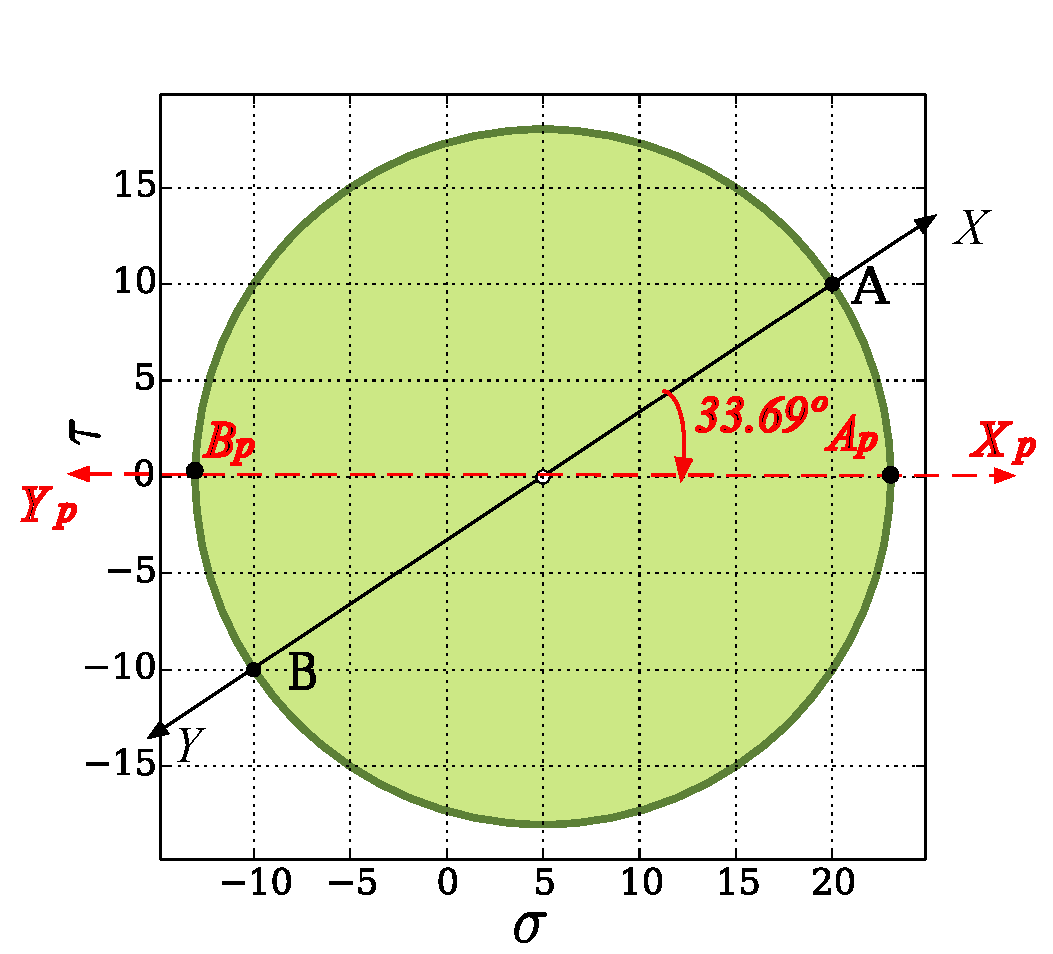
\includegraphics[width=2.5in]{Tens2Prin.pdf}\label{Tens2Prin}}		
	\caption{Círculo de Mohr con valores máximos normales. Puntos $A_p$, $B_p$. }
	\label{TensPrin}
\end{figure}

\begin{figure}[H]
	\centering
		\subfloat [Estado de tensión 1]{ 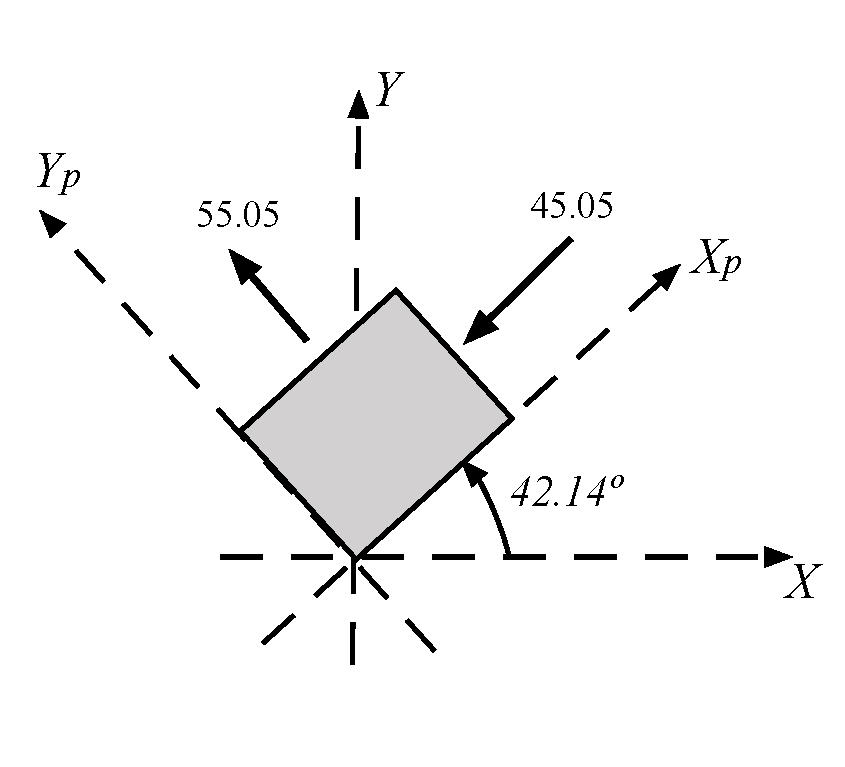
\includegraphics[width=2.5in]{Cubo1Prin.pdf}\label{Cubo1Prin}}
		\hspace{0.5cm}
		\subfloat [Estado de tensión 2]{ 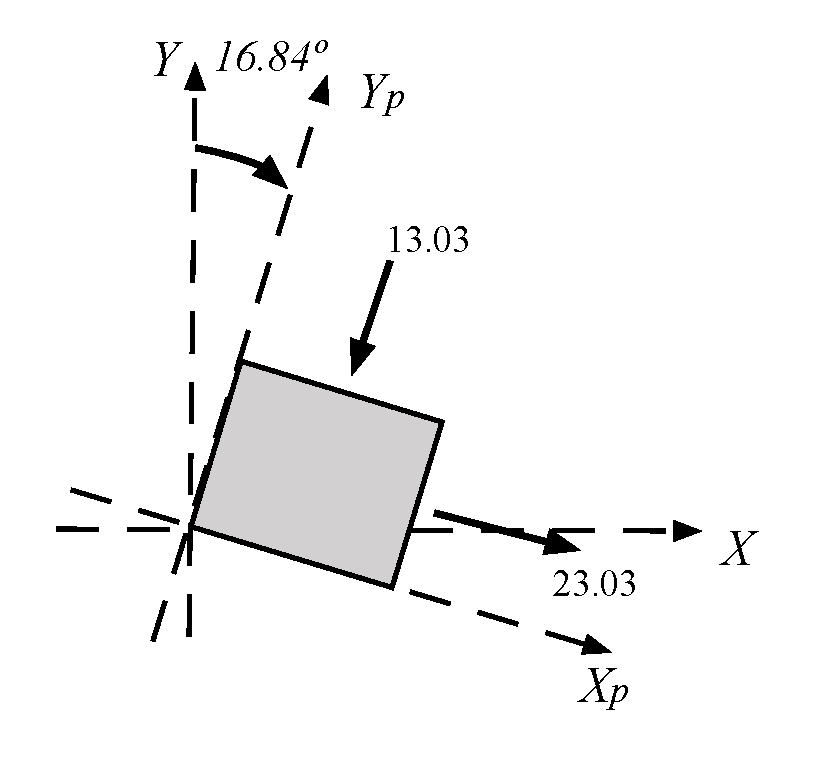
\includegraphics[width=2.5in]{Cubo2Prin.pdf}\label{Cubo2Prin}}		
	\caption{Cubo de tensiones en sistema rotado $x_p-y_p$. }
	\label{CubosPrincipal}
\end{figure}

Nótese que para encontrar el estado principal $1$ rotamos desde el sistema
original $xy$ un ángulo $\alpha = \arctan\left(\dfrac{50}{5}\right)$ en sentido
contrario a las manecillas del reloj, mientras que para el estado principal $2$
rotamos un ángulo $\alpha = \arctan\left(\dfrac{10}{15}\right)$ en sentido de
las manecillas \footnote{La rotación puede ser hecha en cualquier sentido; lo
importante es no perder de vista la ubicación de los ejes y tener en cuenta
que estas rotaciones coinciden en sentido con el problema físico pero que
corresponden a valores de ángulo doble en el círculo}.
Por similitud a la  \cref{cicmohr1} las ecuaciones para encontrar los valores se podrían escribir como:\\
%
\begin {equation}
\begin {aligned}
&\tau^p_{xy} = R \\
&\sigma^p_{xx} = C \pm R \\
&\sigma^p_{yy} = C \mp R  \\
\end {aligned}
\label{cicmohr2}
\end {equation}
%
Los estados de tensiones principales quedarían escritos como:\\
%
 \begin{equation}
[\sigma^p_{1}] =
 	\begin{bmatrix}
     	-45.25 & 0.0 &  \\
     	0.0 & 55.25 \\
 	\end{bmatrix}
 \hspace{1cm}
 [\sigma^p_{2}] =
 	\begin{bmatrix}
     	23.03 & 0.0 &  \\
     	0.0 & -13.03 \\
 	\end{bmatrix}
\end{equation}
%

%
\item[•] Asuma que ambos estados de tensiones ocurren al mismo tiempo y determine
las direcciones principales y valores propios para el estado de tensiones
resultantes. \\\\
%
\textbf{Solución:}
%
Para hacer superposición de los estados de tensiones ambos deben de estar en el
mismo sistema de referencia. En nuestro caso se tiene que inicialemente ambos
están escritos en el mismo sistema de referencia $x y$, por lo que bastará hacer
la suma componente a componente de ambos tensores.
\begin{equation}
[\sigma_t] =
 	\begin{bmatrix}
     	0.0 & -50.0 &  \\
     	-50.0 & 10.0 \\
 	\end{bmatrix}
	+
 	\begin{bmatrix}
     	20.0 & -10.0 &  \\
     	-10.0 & -10.0 \\
 	\end{bmatrix}
 	=
 	\begin{bmatrix}
     	20.0 & -60.0 &  \\
     	-60.0 & 0.0 \\
 	\end{bmatrix}
\end{equation}
%
En la  \cref{TensorSup} se presenta el círculo de Mohr
con el estado original producto de la superposición (linea $X -Y$) y el estado
principal (linea $X_p - Y_p$) mientras que en la \cref{CuboSup} se muestra
el cubo de tensiones del estado principal.
%
\begin{figure}[H]
	\centering
		\subfloat [Circulo de Mohr]{ 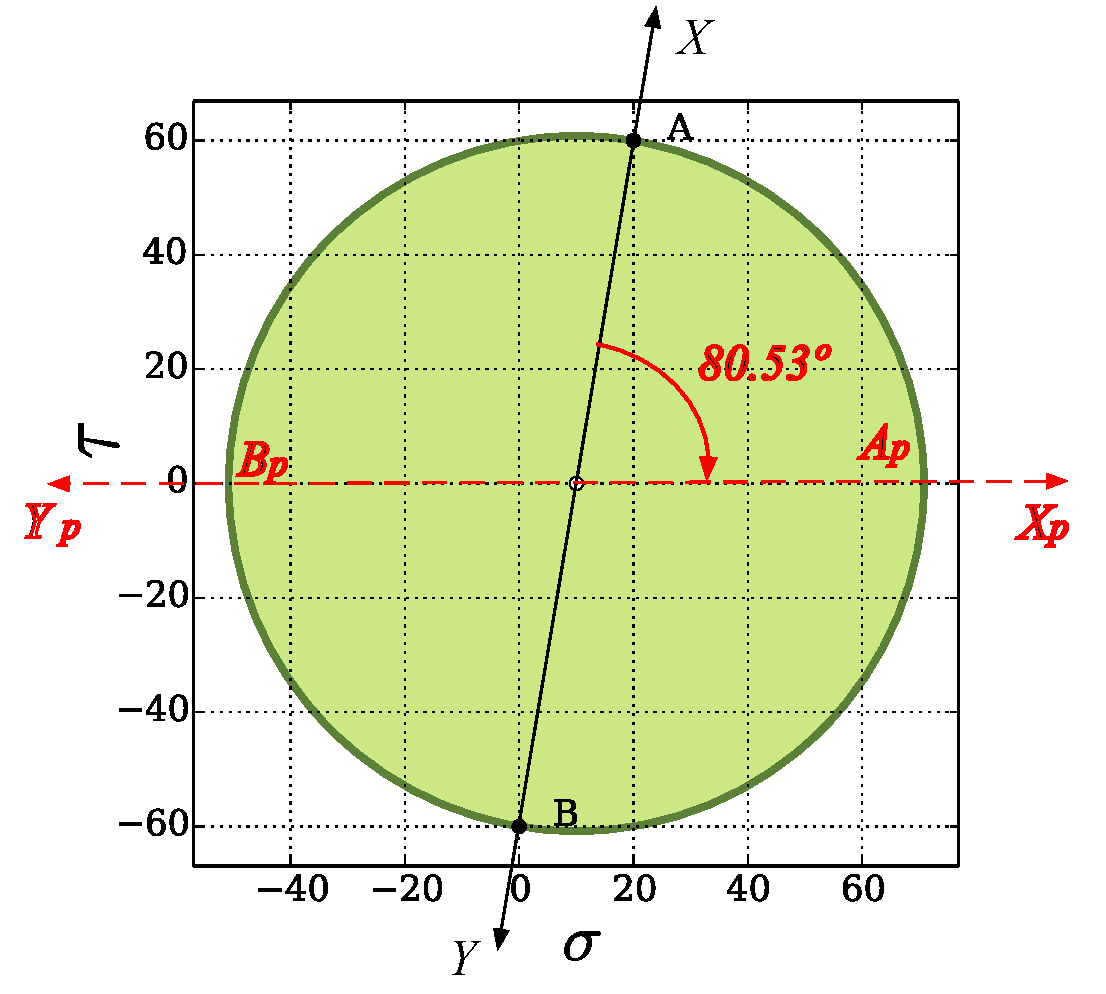
\includegraphics[width=2.5in]{TensorSup.pdf}\label{TensorSup}}
		\hspace{0.5cm}
		\subfloat [Cubo de tensiones]{ 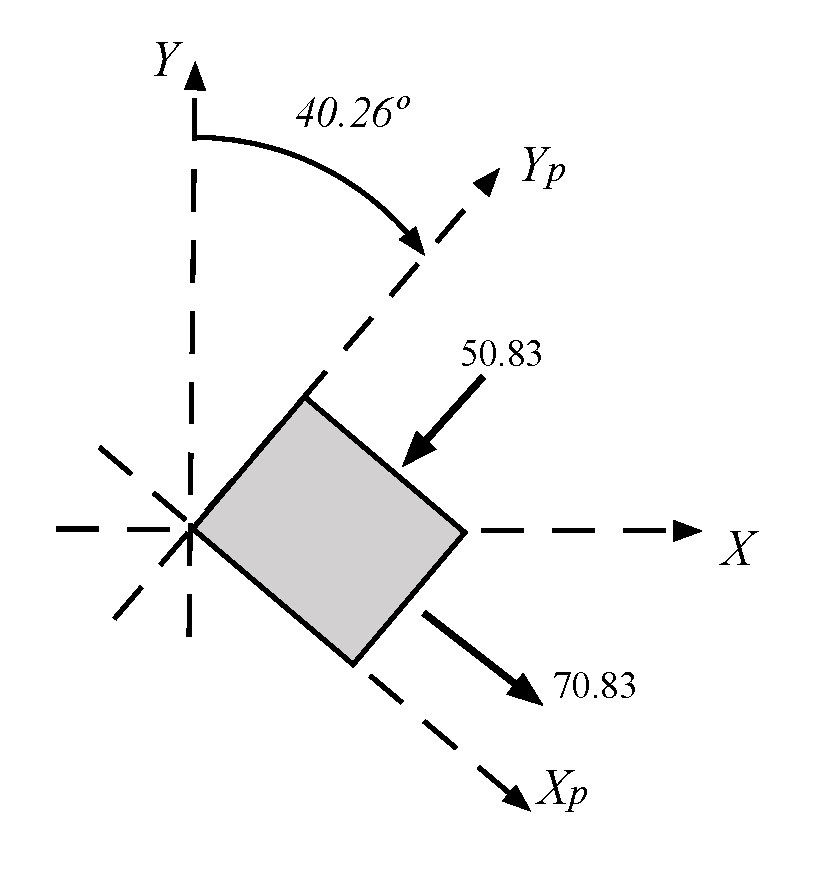
\includegraphics[width=2.5in]{CuboSup.pdf}\label{CuboSup}}		
	\caption{Estado de tension principal superpuesto }
	\label{TensSupPrin}
\end{figure}
%
El tensor escrito en direcciones principales es: 
\begin{equation}
 [\sigma^p_{2}] =
 	\begin{bmatrix}
     	70.83 & 0.0 &  \\
     	0.0 & -50.83 \\
 	\end{bmatrix}
\end{equation}

\end{enumerate}

\subsubsection*{Ejemplo 3: Planos de falla}
Un punto material en un medio continuo est\'a sometido al estado de tensiones mostrado en la \cref{punto}. Si las líneas punteadas corresponden a planos de falla del material y sabiendo que los dos planos {\bf son perpendiculares entre sí}, se pide:

\begin{figure}[H]
	\centering
		\subfloat []{ 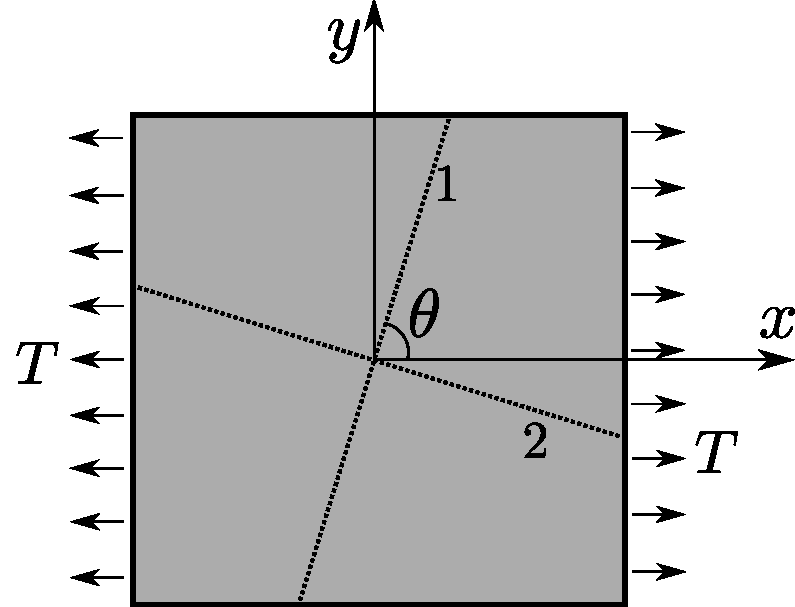
\includegraphics[width=2.5in]{punto.pdf}\label{punto}}		
	\caption{Estado de tensiones}
	\label{punto}
\end{figure}
%
\begin{itemize}

\item[•] Calcular las tensiones normal y tangencial al plano 1.

\textbf{Solución:}\\\\

Escribiendo el estado de tensiones como:

\begin{equation*}
[\sigma]
= 
\begin{bmatrix}
    T & 0 \\
    0 & 0
\end{bmatrix}
\end{equation*}

Para el plano 1 el vector normal es $\hat{n_1}=[ -\sin{\theta}, \cos{\theta} ]$, y la tensi\'on en el plano se calcula como:

\begin{equation*}
t_1 = [\sigma]\hat{n_1}
= 
\begin{bmatrix}
    T & 0 \\
    0 & 0
\end{bmatrix}
\begin{bmatrix}
   -\sin{\theta} \\
    \cos{\theta} \\
\end{bmatrix} \\
\end{equation*}

\begin{equation*}
t_1 = 
\begin{bmatrix}
    -T\sin{\theta} \\
    0 
\end{bmatrix} \\
\end{equation*}

La tensión normal se calcula proyectando la tensión $t_1$ sobre el vector $\hat{n_1}$, 

\begin{equation*}
\sigma_n = 
t_1 \cdot \hat{n_1} = 
\begin{bmatrix}
    -T\sin{\theta} \\
    0 
\end{bmatrix} \cdot
\begin{bmatrix}
    -\sin{\theta} \\
    \cos{\theta} 
\end{bmatrix} \equiv
T\sin^2\theta
\end{equation*}
%
El esfuerzo tangencial se puede calcular proyectando la tensión $t_1$ sobre un vector unitario inscrito en el plano 1. Dando como resultado:

\begin{equation*}
\tau = T\sin{\theta}\cos{\theta} 
\end{equation*}

\item[•] Calcular las tensiones normal y tangencial al plano 2.

\textbf{Solución:}\\\\

Siguiendo un proceso análogo al anterior, se llega a los siguientes resultados:

\begin{equation*}
\sigma_n = T\cos^2\theta 
\end{equation*}

\begin{equation*}
\tau = T\sin{\theta}\cos{\theta}
\end{equation*}

\item[•] Suponiendo que la falla va a ocurrir en alguno o en ambos planos, y que el material es infinitamente resistente a esfuerzos normales, pero no soporta esfuerzos cortantes mayores a $\tau_{adm} = T/4$, calcule el ángulo $\theta$ al cual se produce la falla e indique en cuál plano se presenta la misma. 

\textbf{Solución:}\\\\

\begin{figure}[h]
	\centering
	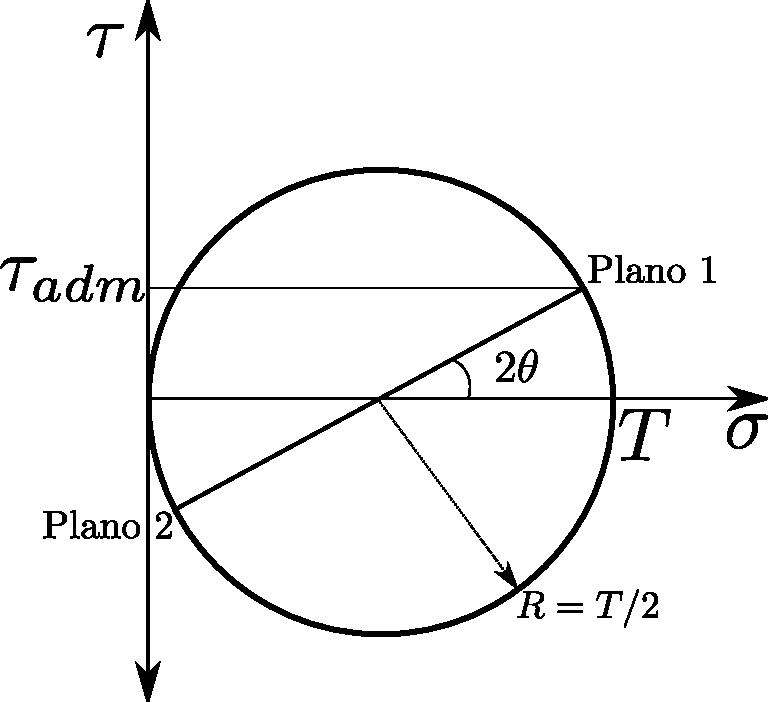
\includegraphics[width=8cm]{sol.pdf} 
	\caption{Circulo de Mohr correspondiente al Estado de tensiones de la \cref{punto}}
	\label{sol}
\end{figure}

Graficando el estado de tensiones como un círculo de Mohr (\cref{sol}), se ubica $\tau_{adm} = T/4$. Luego se llega a la relación:

\begin{equation*}
\sin{2\theta} = \frac{T/4}{T/2} = \frac{1}{2} \rightarrow
\theta = \frac{\pi}{12}
\end{equation*}

La falla se da en cualquier plano, ya que el valor del cortante es igual es ambos por ser perpendiculares.

\end{itemize}


\subsection*{Ejemplo 4: Refuerzo}

Un punto material de un medio continuo se encuentra sometido al estado de tensiones correpondiente al círculo de Mohr de la \cref{estado} y en el cual  $\tau_R$ es la resistencia al corte del material.

\begin{figure}[h]
	\centering
	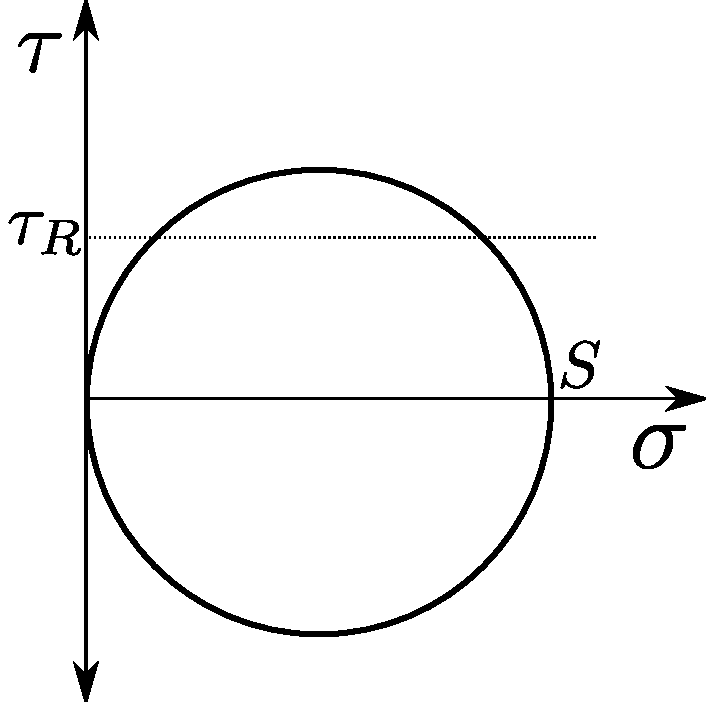
\includegraphics[width=7cm]{estado.pdf} 
	\caption{Estado de tensiones}
	\label{estado}
\end{figure}

Si se requiere aplicar una tracción $S = 3\tau_R$,  proponga una medida de mejoramiento del material, en términos de una aplicación adicional de tensiones, que garantice que éste no falle por cortante.

Del círculo de Mohr, se puede ver que la única manera de evitar que el material falle, es llevándolo a un estado de esfuerzos que no alcance $\tau_R$. En otras palabras, se necesita reducir el radio del círculo de Mohr. La reducción de radio necesaria se muestra en la \cref{modif}. 


\begin{figure}[H]
	\centering
		\subfloat []{ 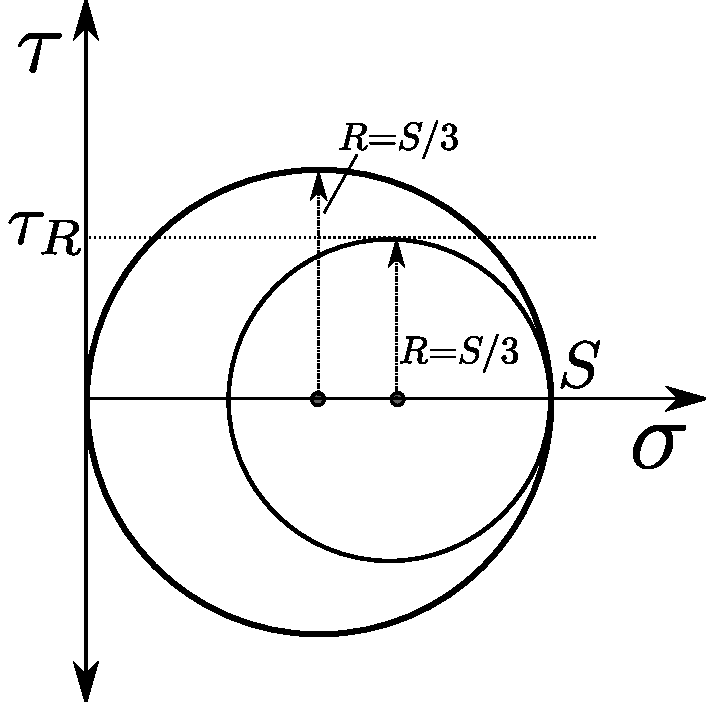
\includegraphics[width=2.5in]{cirmodif.pdf}\label{modif}}		
	\caption{Cambio en el estado de tensiones}
	\label{modif}
\end{figure}

De la \cref{modif} se ve el radio inicial $R=S/2$. El radio del nuevo círculo debe ser $R=S/3$ para que el material no falle por cortante. Entonces


\begin{equation*}
R = \frac{S}{3} =  \frac{\sigma_{xx} - \sigma_{yy}}{2} \rightarrow
\sigma_{yy} = \frac{S}{3}
\end{equation*}

\begin{figure}[h]
	\centering
	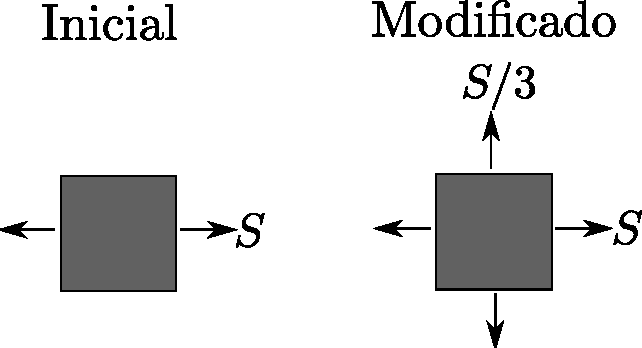
\includegraphics[width=7cm]{estado3.pdf} 
	\caption{Cambio en el estado de tensiones}
	\label{estado3}
\end{figure}

En la \cref{estado3} se ilustra le cambio en las configuraciones de tensiones.


\subsection*{Ejemplo 5: Problema de Cauchy usando Python}
En el enlace: 
%
 {\url{https://github.com/AppliedMechanics-EAFIT/Notas-MMC/blob/master/notebooks/Ej3_Cauchy.ipynb}}
%
\section{Valores y direcciones principales para un estado de tensiones en 3D}
En la sección anterior, para el caso de estados de tensiones en 2 dimensiones (2D), identificamos direcciones o planos trazados por un punto material para los cuales el vector de tracciones solo tenía componente en la dirección normal al plano. Mas aún, se demostró que estas componenetes correspondían a las tensiones máximas y mínimas que experimentaba el punto material. En esta sección se aborda el mismo problema para el caso de estados de tensiones en 3D.  
%
\begin{figure}[H]
\centering
	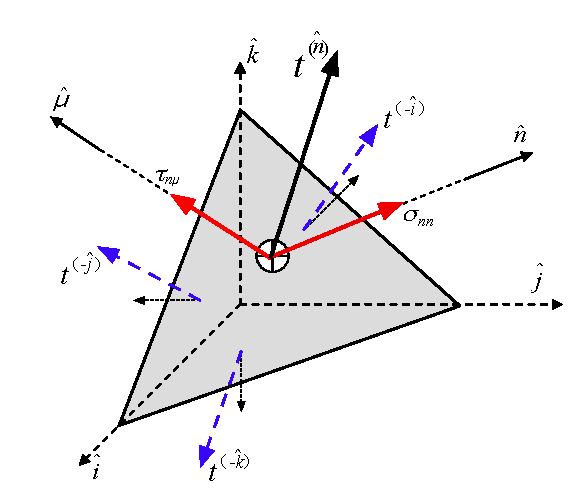
\includegraphics[width=3.5 in]{TetaCauchy.pdf}
	\caption{Elemento diferencial cortado con un plano de vector normal $\hat{n}$ tras lo cual se expone el vector de tracciones ${{\vec t}^{(n)}}$.}
	\label{TetaCauchy}
\end{figure}

Para esto consideremos nuevamente el tetrahedro de Cauchy (\cref{TetaCauchy}) representando el estado de tensiones en un punto material del medio continuo. Sobre este se traza un plano con vector normal externo $\hat{n}$. Adicionalmente, sobre este plano también trazamos un vector ${\hat \mu }$ contenido en el plano inclinado. De otro lado, el vector de tracciones asociado con el plano inclinado se denota como ${\vec t^{(\hat n)}}$. Nótese que el vector de tracciones y el vector normal $\hat{n}$ no son colineales.

En la \cref{incltract} el vector de tracciones se escribe en términos de sus componentes normal y paralela al plano, denotadas como ${\sigma _{nn}}$ y ${\tau _{n\mu }}$ respectivamente.
%
\begin{equation}
{{\vec t}^{(\hat n)}} = {\sigma _{nn}}\hat n + {\tau _{n\nu }}\hat \nu.
\label{incltract}
\end{equation}

De la representación anterior claramente se identifica que la máxima componente normal ${\sigma _{nn}}$ se presenta cuando las direcciones de ${\vec t^{(\hat n)}}$ y $\hat{n}$ coincidan, en cuyo caso podemos escribir;

\begin{equation}
{{\vec t}^{(\hat n)}} = \tilde \sigma \hat n
\label{Cauchyescalar}
\end{equation}

donde ${\tilde \sigma }$ representa dicho valor máximo. De otro lado, tenemos que el vector ${\vec t^{(\hat n)}}$ también puede ser encontrado a partir del tensor de tensiones y de la dirección $\hat{n}$ a través de la fórmula de Cauchy escrita en notación matricial como;

\begin{equation}
\left\{ {{t^{(\hat n)}}} \right\} = \left[ \sigma  \right]\left\{ {\hat n} \right\}.
\label{CauchyO}
\end{equation}

Comparando la \cref{Cauchyescalar} con la \cref{CauchyO} podemos escribir;

\begin{equation}
\left[ {\sigma  - \tilde \sigma I} \right]\left\{ {\hat n} \right\} = \left\{ 0 \right\}
\label{eigen}
\end{equation}

el cual corresponde a un problema de autovalores para la matriz de esfuerzos. Este problema tiene una solución no trivial ($\hat{n}\neq 0$) cuando;

\[\det \left[ {\sigma  - \tilde \sigma I} \right] = 0.\]

En foma expandida escribimos;

\[\det \left[ {\begin{array}{*{20}{c}}
{{\sigma _{xx}} - \tilde \sigma }&{{\tau _{xy}}}&{{\tau _{xz}}}\\
{{\tau _{yx}}}&{{\sigma _{yy}} - \tilde \sigma }&{{\tau _{yz}}}\\
{{\tau _{zx}}}&{{\tau _{zy}}}&{{\sigma _{zz}} - \tilde \sigma }
\end{array}} \right] = 0\]

y evaluando el determinante se tiene;
\begin{align}
{{\tilde \sigma }^3} - ({\sigma _{xx}} + {\sigma _{yy}} + {\sigma _{zz}}){{\tilde \sigma }^2} + ({\sigma _{xx}}{\sigma _{yy}} + {\sigma _{xx}}{\sigma _{zz}} + {\sigma _{zz}}{\sigma _{yy}} - \tau _{xy}^2 - \tau _{xz}^2 - \tau _{yz}^2)\tilde \sigma  - \nonumber \\
 ({\sigma _{xx}}{\sigma _{yy}}{\sigma _{zz}} + 2{\tau _{xy}}{\tau _{xz}}{\tau _{yz}} - {\sigma _{xx}}\tau _{yz}^2 - {\sigma _{yy}}\tau _{xz}^2 - {\sigma _{zz}}\tau _{xy}^2) = 0.
\label{caracteristica}
\end{align}

\begin{itemize}
\item[•] La \cref{caracteristica} corresponde a la ecuación  característica del problema de autovalores dado en \cref{eigen}.
\item[•] Dado que el tensor de tensiones es simétrico y real su ecuación característica tiene 3 raices reales distintas denotadas como ${{\tilde \sigma }_1}$, ${{\tilde \sigma }_2}$ y ${{\tilde \sigma }_3}$ y tales que ${{\tilde \sigma }_1} \geq{{\tilde \sigma }_2} \geq {{\tilde \sigma }_3}$.
\item[•] Los valores principales ${{\tilde \sigma }_1}$, ${{\tilde \sigma }_2}$ y ${{\tilde \sigma }_3}$ corresponden a las tensiones máxima, intermedia y mínima que experimenta el punto material. 
\item[•] Para cada raíz (tensión extrema) de la ecuación característica existe una dirección asociada $\hat{n}$ la cual se encuentra usando la \cref{eigen} y la condición $n_x^2 + n_y^2 + n_z^2 = 1.$
\end{itemize}

De otro lado, considerando que le \cref{caracteristica} da como solución las tensiones principales ${{\tilde \sigma }_1}$, ${{\tilde \sigma }_2}$ y ${{\tilde \sigma }_3}$ necesariamente se tiene que los coeficientes deben ser independientes del sistema de referencia en que se tenga el tensor de tensiones. De lo anterior se tiene que la ecuación característica se puede escribir como;

\[{{\tilde \sigma }^3} - {I_\sigma }{{\tilde \sigma }^2} + I{I_\sigma }\tilde \sigma  - II{I_\sigma } = 0\]

donde;

\[{I_\sigma } = {\sigma _{xx}} + {\sigma _{yy}} + {\sigma _{zz}}\]
\[I{I_\sigma } = {\sigma _{xx}}{\sigma _{yy}} + {\sigma _{xx}}{\sigma _{zz}} + {\sigma _{zz}}{\sigma _{yy}} - \tau _{xy}^2 - \tau _{xz}^2 - \tau _{yz}^2\]
\[II{I_\sigma } = {\sigma _{xx}}{\sigma _{yy}}{\sigma _{zz}} + 2{\tau _{xy}}{\tau _{xz}}{\tau _{yz}} - {\sigma _{xx}}\tau _{yz}^2 - {\sigma _{yy}}\tau _{xz}^2 - {\sigma _{zz}}\tau _{xy}^2\]

son constantes independientes del sistema de referencia\footnote{Estas constantes se denominan los invariantes del tensor de tensiones y juegan un papel análogo a la magnitud de un vector la cual permanece constante independientemente del sistema de referencia en el que se escriba el vector}.

%\textbf{•}\subsection*{Ejemplo 6: cálculo de valores principales}
%\footnote{Este ejemplo ha sido implementado en el siguiente notebook de Python http://nbviewer.ipython.org/urls/dl.dropbox.com/s/0bnyl2qvauk85i2/Ej4\_Eingen.ipynb}
Consideremos el siguiente estado de tensiones con componentes correspondientes a un sistema de referencia $x-y-z$;

\[\sigma  = \left[ {\begin{array}{*{20}{c}}
{200}&{100}&{300}\\
{100}&0&0\\
{300}&0&0
\end{array}} \right].\]

Se pide determinar las tensiones principales y sus direcciones asociadas.

La ecuación característica esta dada por;

\[{{\tilde \sigma }^3} - 200{{\tilde \sigma }^2} - 100000\tilde \sigma  = 0\]

donde identificamos los 3 invariantes como;


\[{I_\sigma } = 200\]
\[I{I_\sigma } =  - 100000\]
\[II{I_\sigma } = 0.\]
%
Resolviendo la ecuación característica determinamos las tensiones principales ${{\tilde \sigma }_1} = 432$, ${{\tilde \sigma }_2} = 0$ y ${{\tilde \sigma }_3} =  - 232$.

La dirección asociada con la tesion ${{\tilde \sigma }_1} = 432$ resulta de resolver;

\[\left[ {\begin{array}{*{20}{c}}
{ - 232}&{100}&{300}\\
{100}&{ - 432}&0\\
{300}&0&{ - 432}
\end{array}} \right]\left\{ {\begin{array}{*{20}{c}}
{{n_x}}\\
{{n_y}}\\
{{n_z}}
\end{array}} \right\} = \left\{ {\begin{array}{*{20}{c}}
0\\
0\\
0
\end{array}} \right\}\]

y

\[n_x^2 + n_y^2 + n_z^2 = 1.\]

De la segunda y tercera ecuación se tiene;

\[{n_y} = \frac{{100}}{{432}}{n_x}\]

y

\[{n_z} = \frac{{300}}{{432}}{n_x}.\]

Usando estas en $n_x^2 + n_y^2 + n_z^2 = 1$ se tiene que;

\[{n_x} =  \pm 0.807\]

mientras que ${n_y} = 0.187$ y ${n_z} = 0.560$. Por lo tanto la dirección asociada con la tensión principal ${{\tilde \sigma }_1} = 432$ corresponde al vector ${{\hat n}^1} = 0.807\hat i + 0.187\hat j + 0.560\hat k$.

Similarmente, resolviendo para ${{\tilde \sigma }_2} = 0$ se tiene;


\[\left[ {\begin{array}{*{20}{c}}
{ 200}&{100}&{300}\\
{100}&{ 0}&0\\
{300}&0&{0}
\end{array}} \right]\left\{ {\begin{array}{*{20}{c}}
{{n_x}}\\
{{n_y}}\\
{{n_z}}
\end{array}} \right\} = \left\{ {\begin{array}{*{20}{c}}
0\\
0\\
0
\end{array}} \right\}\]

De la segunda (o la tercera) ${n_x} = 0$ mientras que de la primera ${n_y} =  - 3{n_z}$. Finalmente de la condición $n_x^2 + n_y^2 + n_z^2 = 1$ se tiene que la dirección asociada con la tensión principal ${{\tilde \sigma }_2} = 0$ corresponde a ${{\hat n}^2} =-948\hat j + 0.316\hat k$.
%
Finalmente para la tensión principal ${{\tilde \sigma }_3} =  - 232$ resolvemos;

\[\left[ {\begin{array}{*{20}{c}}
{ 432}&{100}&{300}\\
{100}&{ 232}&0\\
{300}&0&{232}
\end{array}} \right]\left\{ {\begin{array}{*{20}{c}}
{{n_x}}\\
{{n_y}}\\
{{n_z}}
\end{array}} \right\} = \left\{ {\begin{array}{*{20}{c}}
0\\
0\\
0
\end{array}} \right\}.\]

De la segunda y la tercera se tiene que ${n_y} =  - \frac{{100}}{{231}}{n_x}$ y ${n_z} =  - \frac{{300}}{{231}}{n_x}$  mientras que de la condición $n_x^2 + n_y^2 + n_z^2 = 1$ se tiene que la dirección asociada con la tensión principal ${{\tilde \sigma }_3} = -232$ corresponde a ${{\hat n}^3} = 0.592\hat i - 0.255\hat j - 0.766\hat k$.

Nótese que en el paso final del cálculo de las direcciones principales ${{\hat n}^1}$, ${{\hat n}^2}$ y ${{\hat n}^3}$ se uso la condicíon $n_x^2 + n_y^2 + n_z^2 = 1$ para determinar una de las componentes a partir de las cuales era posible determinar las 2 restantes.

Por ejemplo en el caso de ${{\tilde \sigma }_1} = 432$ esta condición arrojó como resultado ${n_x} =  \pm 0.807$. Para determinar las componentes ${n_y}$ y ${n_z}$ usamos las relaciones ${n_y} = \pm \frac{{100}}{{432}}{n_x}$ y ${n_z} = \pm \frac{{300}}{{432}}{n_x}$ sobre las cuales trasladamos los 2 posibles signos de ${n_x}$. Lo anterior indica que las direcciones principales corresponden a vectores con direcciones opuestas lo cual es equivalente a observar de manera simultanea las tracciones sobre la dirección positiva y negativa del punto material. Por ejemplo, en el caso de la tensión principal ${{\tilde \sigma }_1} = 432$ obtenemos las direcciones ${{\hat n}^1} = 0.807\hat i + 0.187\hat j + 0.560\hat k$ y su opuesta ${{-\hat n}^1} = -0.807\hat i - 0.187\hat j - 0.560\hat k$.
%
\subsubsection{Tarea}
Comprobar la ortogonalidad de las direcciones principales.
Transformar el tensor de tensiones al sistema de referencia determinado por las direcciones principales y verificar que el tensor se diagonaliza en dicha dirección. 

\subsection{Circulo de Mohr en 3D}

Con los tres valores principales ${{\tilde \sigma }_1}$, ${{\tilde \sigma }_2}$ y  ${{\tilde \sigma }_3}$ es posible realizar una representación plana del problema de tensión en 3D tal y como se muestra en \cref{Mohr3D}. Estos circulos tienen centro y radio dados por;

\begin{align*}
\sigma _c^I & = \frac{{{{\tilde \sigma }_1} + {{\tilde \sigma }_3}}}{2} \\
\sigma _c^{II} & = \frac{{{{\tilde \sigma }_1} + {{\tilde \sigma }_2}}}{2} \\
\sigma _c^{III} & = \frac{{{{\tilde \sigma }_2} + {{\tilde \sigma }_3}}}{2}
\end{align*}

\begin{align*}
{R_I}& = \frac{{{{\tilde \sigma }_1} - {{\tilde \sigma }_3}}}{2}\\
{R_{II}}& = \frac{{{{\tilde \sigma }_1} - {{\tilde \sigma }_2}}}{2}\\
{R_{III}}& = \frac{{{{\tilde \sigma }_2} - {{\tilde \sigma }_3}}}{2}
\end{align*}

Es claro que para poder graficar el círculo de Mohr en 3D es necesario resolver primero el problema de tensiones y direcciones principales. Aunque una vez disponible, el círculo se puede usar para localizar el estado de tensiones en otras direcciones (intersección de los 3 radios) por el momento solo se hará uso del mismo para calcular el cortante máximo.


\begin{figure}[H]
\centering
	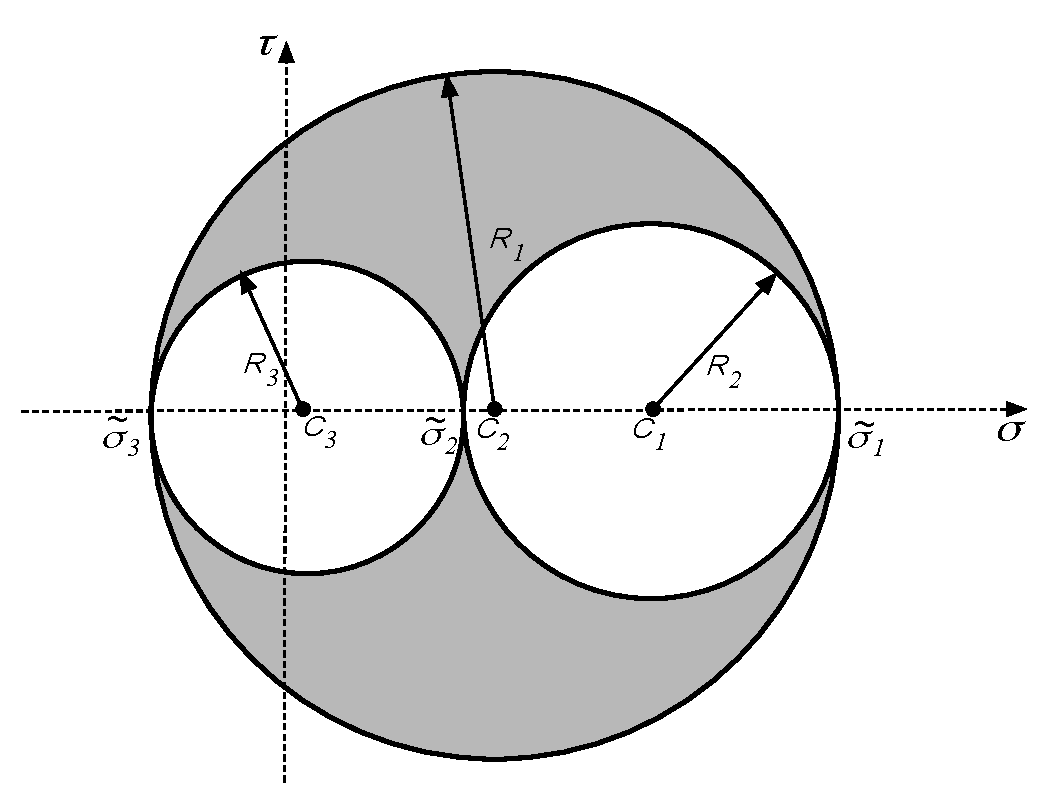
\includegraphics[width=4.0 in]{Mohr3d.pdf}
	\caption{Círculo de Mohr}
	\label{Mohr3D}
\end{figure}

De \cref{Mohr3D} es importante resaltar que el esfuerzo cortante máximo está dado por:

\[\tau_{max} =\frac{{\tilde \sigma }_1 - {\tilde \sigma }_3}{2} \]


\section{Ejercicios}

\begin{enumerate}
\item \label{punto01} La \cref{figura2:mala} muestra el estado de tensión
en un punto $P$ del Medio Continuo para varias direcciones: \footnote{Tomado del problema 3.12 en Chávez, E. Problemas resueltos de mecánica del medio Continuo}

\begin{figure}[H]
	\centering
	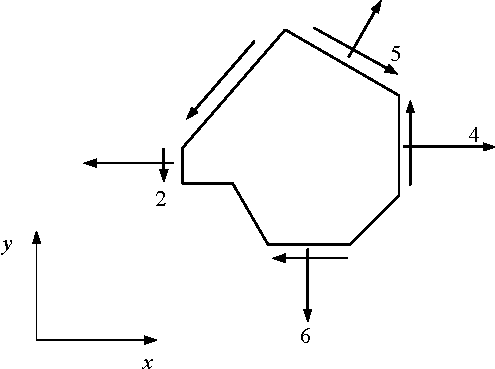
\includegraphics[width=8cm]{Ejer3_1.pdf}
	\caption{Estado de tensiones en el punto en diferentes direcciones.}
	\label{figura2:mala}
\end{figure}
\begin{enumerate}
	\item Obtener el estado de tensiones $[\sigma]$ en el punto $P$ del Medio
	Continuo.
	\item Representar el estado de tensiones mediante el c\'irculo de Mohr.
	\item Hallar las tensiones normales m\'aximas y la direcci\'on en la que se presentan.
	\item Utilizando el círculo de Mohr, hallar las tensiones cortantes m\'aximas y la direcci\'on en la que se presentan.
	\item Encontrar el estado de tensiones en un sistema de referencia cartesiano que se encuentra rotado $30^{0}$ respecto al sistema mostrado en la figura.
	\item En la  \cref{figura2:mala} uno de los valores de corte presentado no es correcto. \textquestiondown  Diga cual es y por que?
\end{enumerate}

\item \label{punto02} Las componentes del tensor de tensiones es un punto $P$
son:
		\[{[\sigma]} = \left[ \begin{array}{ccc}
		1 & 2 & 3 \\ 
		2 & 4 & 6 \\ 
		3 & 6 & 1
		\end{array}  \right] \enspace\]
%
Encontrar:
%
\begin{enumerate}
	\item El vector de tracci\'on $\mathbf{t}$ en $P$ para un plano normal al eje $x_1$;
	\item El vector de tracci\'on $\mathbf{t}$ en $P$ para un plano cuya normal es $\frac{1}{\sqrt{6}}(1,-1,2)$;
	\item El vector de tracci\'on $\mathbf{t}$ en $P$ para el plano $2x_1 - 2x_2 - x_3 = 0$;
\end{enumerate}

\item \label{punto03} La  \cref{planos} muestra dos estados de tensiones
para el mismo punto de un medio continuo. \footnote{Tomado del problema 4.8 en Reddy, J.N (2010). An introduction to continuum mechanics}
%
\begin{figure}[H]
	\centering
	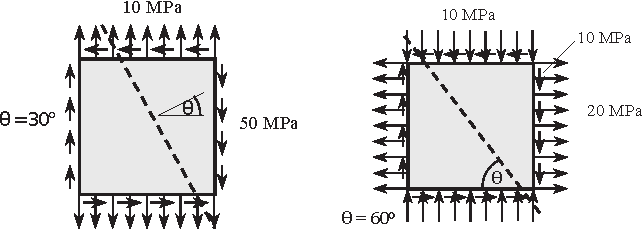
\includegraphics[width=12cm]{Ejer3_3.pdf}
	\caption{Estado de tensiones en un punto.}
	\label{planos}
\end{figure}
	%
\begin{enumerate}
	\item Determinar los esfuerzos normales sobre los planos mostrados con linea punteada en las figuras para cada uno de los estados.
	\item Determinar los esfuerzos cortantes sobre los planos mostrados con linea punteada en las figuras para cada uno de los estados.
	\item Para cada uno de los estados de tensiones mostrados determinar los valores propios y las direcciones principales.
	\item Asuma que ambos estados de tensiones ocurren al mismo tiempo y determine las direcciones principales y valores propios para el estado de tensiones resultantes.
	\item Para el estado de tensiones resultante de sumar los estados mostrados, determinar el estado de tensiones en un sistema de referencia que se encuentra a $90^0$ del mostrado en la figura.
	\item Para el estado de tensiones resultante de sumar los estados mostrados, determinar el estado de tensiones en un sistema de referencia que se encuentra a $180^0$ del mostrado en la figura.
	\item Para el estado de tensiones resultante de sumar los estados mostrados, determinar el estado de tensiones en un sistema de referencia que se encuentra a $270^0$ del mostrado en la figura.
	\item Para el estado de tensiones resultante de sumar los estados mostrados, determinar el estado de tensiones en un sistema de referencia que se encuentra a $45^0$ del mostrado en la figura.
\end{enumerate}

\item \label{punto04} La  \cref{caras} muestra un cuerpo sometido a
diferentes tensiones en la superficie del mismo. Escribir el vector de tensiones
en cada una de la superficies del medio continuo. \footnote{Tomado del problema 4.2 en Reddy, J.N (2010). An introduction to continuum mechanics}
%
\begin{figure}[H]
	\centering
	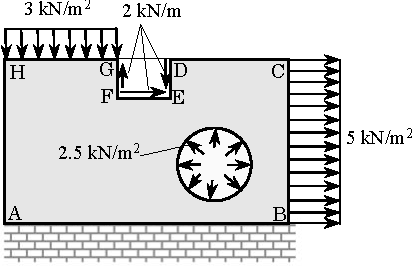
\includegraphics[width=7cm]{Ejer3_4.pdf}
	\caption{Medio Continuo sometido a diferentes tensiones en su superficie.}
	\label{caras}
\end{figure}	
% *************************** %
\item \label{punto05} En la  \cref{cuna:tensiones} se dan las tensiones
$\vec{t}_1$ y $\vec{t}_2$ en dos planos no perpendiculares:\\
%	
\begin{figure}[H]
	\centering
	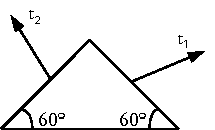
\includegraphics[width=6cm]{Ejer3_5.pdf}
	\caption{Estado de tensiones en un punto.}
	\label{cuna:tensiones}
\end{figure}
\begin{enumerate}
	\item Hallar el tensor de tensiones $[\sigma]$ en el sistema $x-y$ (horizontal y vertical), si \begin{large} $\vec{t}_1= 4 \hat{i} + 2 \sqrt{3} \hat{j}$ \end{large} y  \begin{large} $\vec{t}_2= -2 \hat{i} +0 \hat{j}$ \end{large}.\\
\end{enumerate}

\item \label{punto06} La \cref{direcc} muestra dos estados de tensiones
para el mismo punto de un medio continuo. 
%
\begin{figure}[H]
	\centering
	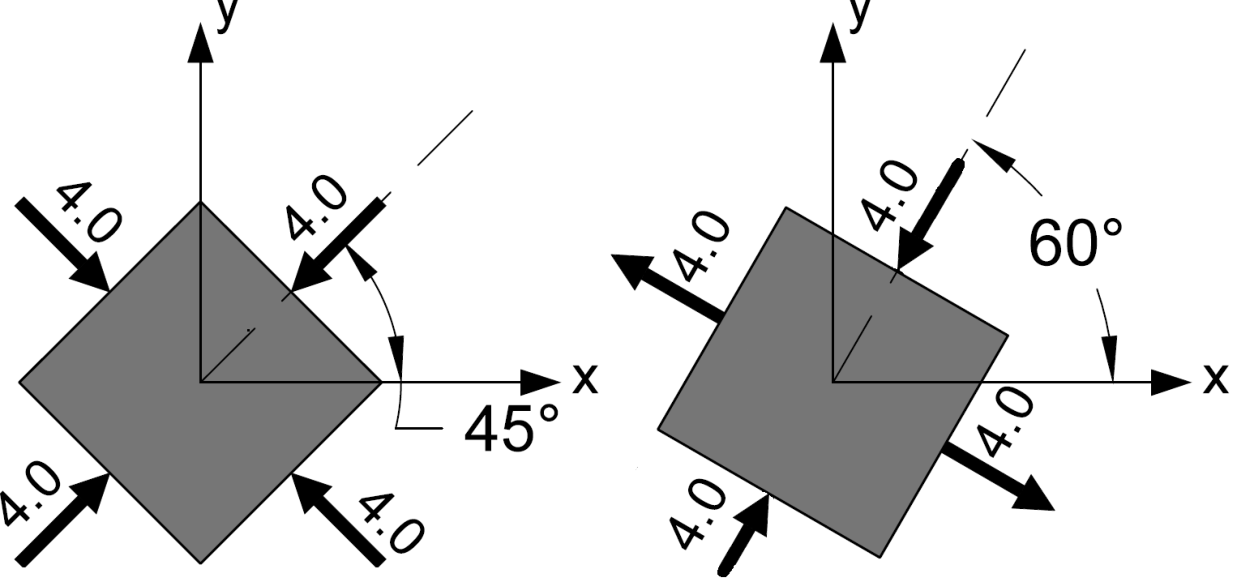
\includegraphics[width=9cm]{Ejer3_6.pdf}
	\caption{Estados de tensiones en un punto.}
	\label{direcc}
\end{figure}
%
\begin{enumerate}
	\item Para cada uno de los estados de tensiones mostrados determinar los
valores propios y las direcciones principales.
	\item Asuma que ambos estados de tensiones ocurren al mismo tiempo y determine
las direcciones principales y valores propios para el estado de tensiones resultantes.
	\item Para el estado de tensiones resultante de sumar los estados mostrados,
determinar el estado de tensiones en un sistema de referencia que se encuentra a $90^0$ del mostrado en la figura.
	\item Para el estado de tensiones resultante de sumar los estados mostrados,
determinar el estado de tensiones en un sistema de referencia que se encuentra a $180^0$ del mostrado en la figura.
	\item Para el estado de tensiones resultante de sumar los estados mostrados,
determinar el estado de tensiones en un sistema de referencia que se encuentra a $270^0$ del mostrado en la figura.
	\item Para el estado de tensiones resultante de sumar los estados mostrados,
determinar el estado de tensiones en un sistema de referencia que se encuentra a $45^0$ del mostrado en la figura.
\end{enumerate}
%

% *************************** %
\item \label{punto07} El tensor de tensiones en el punto $P$ est\'a definido
como
%	
		\[{[\sigma]} = \left[ \begin{array}{ccc}
		8 & -4 & 1 \\ 
		-4 & 3 & 0.5 \\ 
		1 & 0.5 & 2
		\end{array}  \right] \enspace\]
	%
Calcular el vector de tracci\'on en el punto $P$ seg\'un la normal del plano ABC
(ver figura \cref{norplano}) y descompongalo en su componente normal y tangencial
%
\begin{figure}[H]
	\centering
	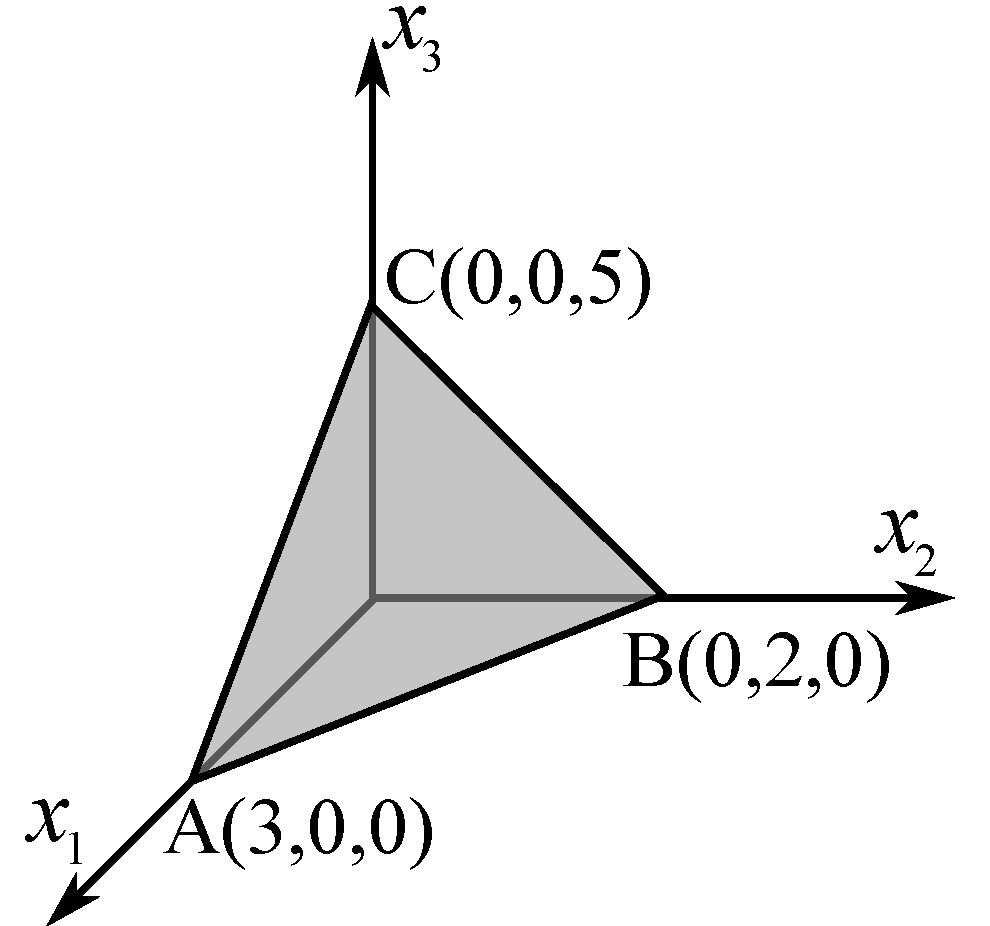
\includegraphics[width=7.5cm]{Ejer3_7.pdf}
	\caption{}
	\label{norplano}
\end{figure}
% *************************** %
\item \label{punto08} Escribir el tensor de tensiones y hacer la
representaci\'on en el c\'irculo de Mohr para los siguientes caso:
%
\begin{enumerate}
	\item Caso unidimensional, estado de carga de tracci\'on.
	\item Caso unidimensional, estado de carga de compresi\'on.
	\item Caso bidimensional, estado de carga de tracci\'on.
	\item Caso bidimensional, estado de corte puro.
\end{enumerate}
% *************************** %
\item \label{punto09} Para un prisma rectangular con secci\'on transversal $A$,
calcular el tensor de esfuerzos de Cauchy en un punto en el interior si se somete a una fuerza $f$ distribuida uniformemente en la parte superior (ver \cref{prisma}). 
Para $A=1$ $m^2$ y $f=1000$ $kgf/m^2$ calcular el valor
y la direcci\'on de los cortantes m\'aximos.\\
%
\begin{figure}[H]
	\centering
	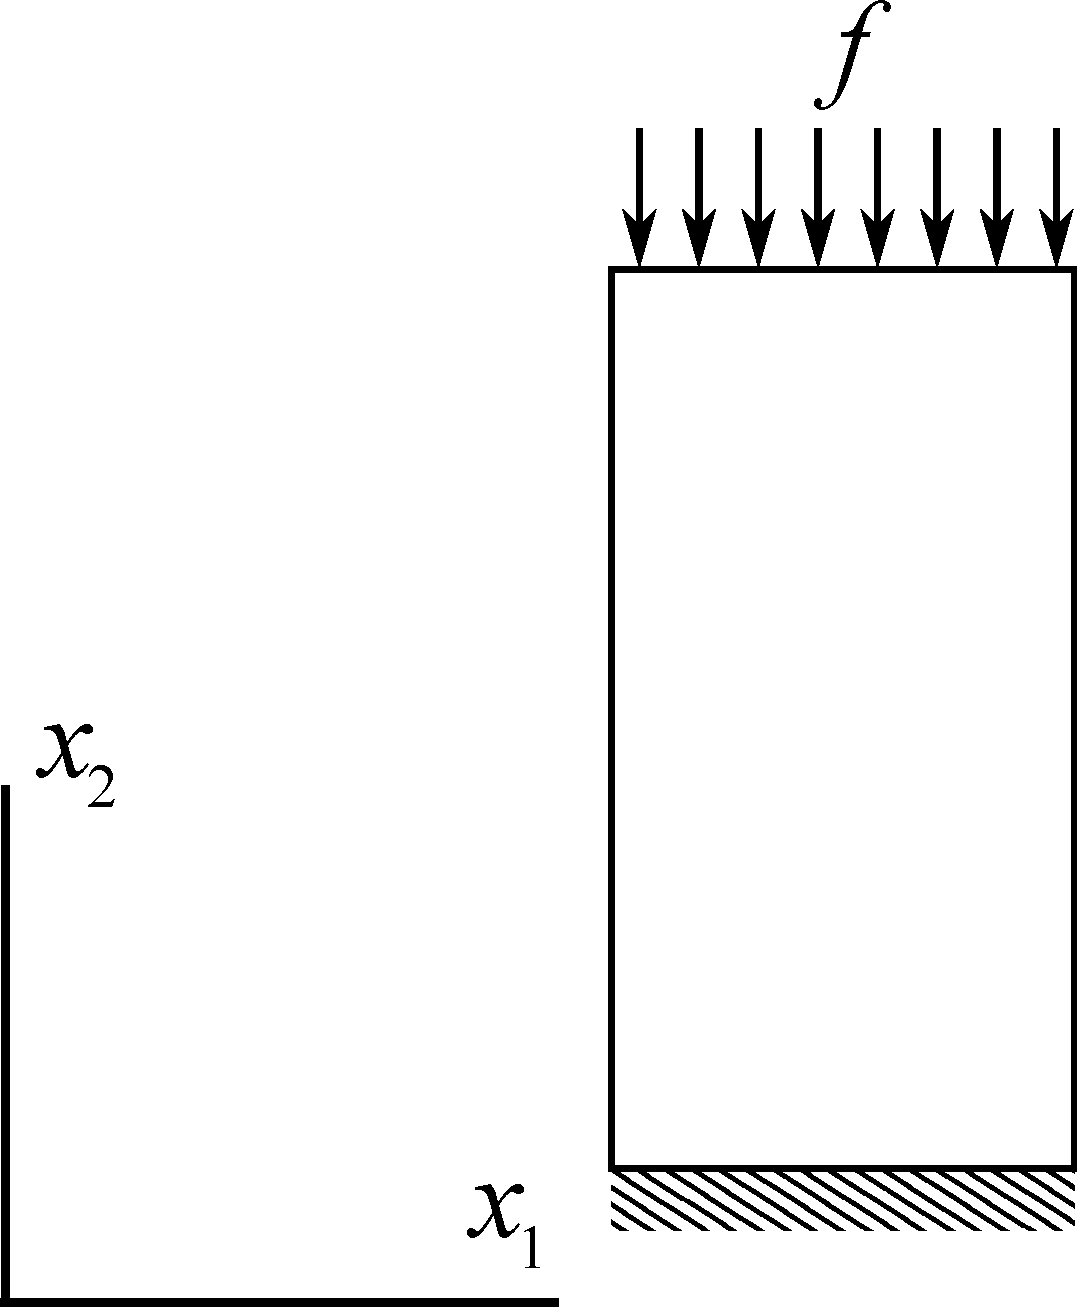
\includegraphics[width=5cm]{Ejer3_9.pdf}
	\caption{}
	\label{prisma}
\end{figure}
% *************************** %
\item \label{punto10} En la \cref{super:cuna-square} se dan las tensiones
para un mismo punto asociados a dos estados I y II. Determinar el estado de tensiones III si el estado I y II ocurren al mismo tiempo. \footnote{Tomado del ejemplo 4.4 en Olivella, X; Saracíbar, C (2000). Mecánica de Medios Continuos para ingenieros}\\
%
\begin{figure}[H]
	\centering
	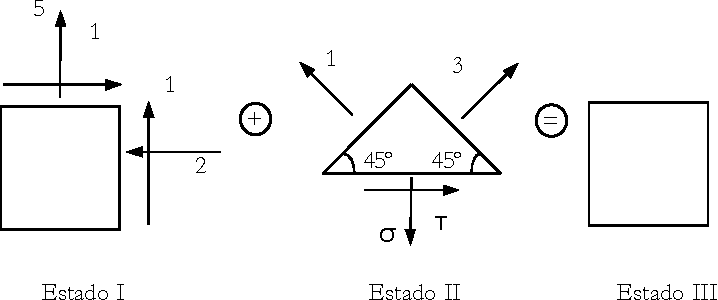
\includegraphics[width=11cm]{Ejer3_10.pdf}
	\caption{Estado de tensiones en un punto.}
	\label{super:cuna-square}
\end{figure}
%
% *************************** %
\item \label{punto11} La \cref{compresimple} corresponde al montaje
de la prueba de laboratorio de compresi\'on simple usada para determinar la resistencia del concreto.\\
%
\begin{figure}[H]	
	\centering	
	\subfloat [Ensayo de compresi\'on simple]{ 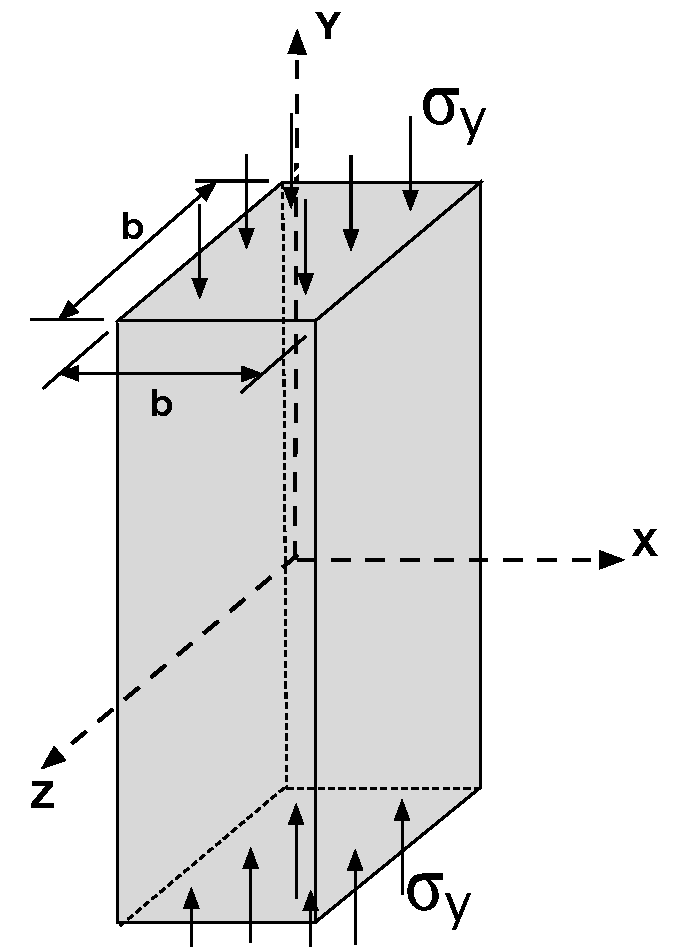
\includegraphics[width=2.2in]{Ejer3_11_1.pdf}\label{compresimple}}
	\hspace{10mm}
	\subfloat [Sección en planta de lado $b$, ensayo confinado]{ 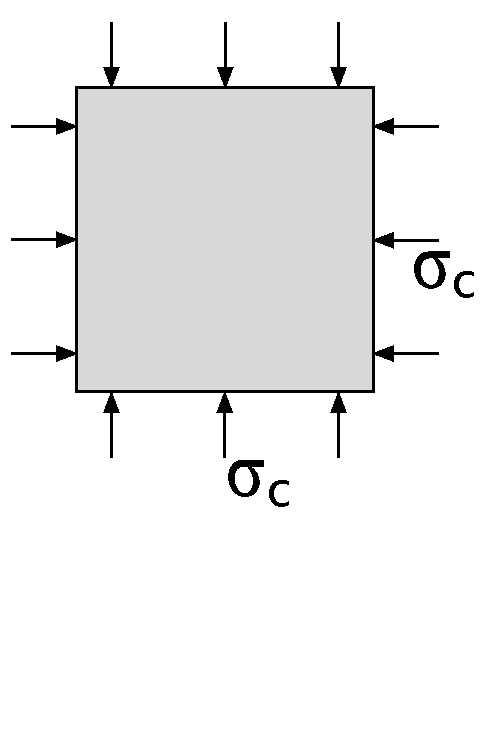
\includegraphics[width=1.8in]{Ejer3_11_2.pdf}\label{compreconf}}
	\caption{Columna en ensayo de compresión}
\end{figure}
%
\begin{enumerate}
	\item Hallar la tensión normal $\sigma_y$ m\'inima que produce la falla a cortante en el modelo presentado en la \cref{compresimple}, sabiendo que la capaciad m\'axima del material ante esfuerzos de corte es $\tau_{max}=A$.
	\item Chequear el equilibrio diferencial (local) de la probeta del ensayo.
	\item Si ahora se hace el mismo ensayo pero con confinamiento perimetral como el mostrado en la \cref{compreconf}, determine el valor minimo del esfuerzo de confinamiento $\sigma_c$ para obtener un un  esfuerzo axial máximo $\sigma_y = 10A$ y un cortante máximo  $\tau_{max}=A$.
\end{enumerate}

% *************************** %
\item \label{punto12} En la \cref{bloque} se muestra un bloque macizo de
arcilla que se extrajo temporalmente de un muro estructural.Por efecto de funcionamiento del muro, todos los puntos al interior del bloque se ven sometidos al estado de esfuerzos presentado en la \cref{esfuerzo}.
%
\begin{figure}[H]
	\centering
		\subfloat [Bloque macizo de arcilla extraido del muro estructural]{ 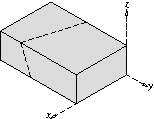
\includegraphics[width=2.5in]{Ejer3_12_1.pdf}\label{bloque}}
		\hspace{0.5cm}
		\subfloat [Esfuerzos en cualquier punto del bloque $(kgf/cm^2)$.]{ 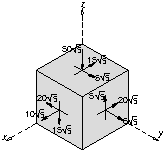
\includegraphics[width=2.5in]{Ejer3_12_2.pdf}\label{esfuerzo}}		
	\caption{ }
	\label{TensSupPrin}
\end{figure}
%
Para examinar el bloque, este fue cortado como se muestra en la \cref{corte} , y para colocarlo nuevamente en el muro, las dos piezas en que fue dividido se unirán con un pegamento, que con el tiempo incrementa su resistencia ante esfuerzos tangenciales y esfuerzos de tracción, tal como se muestra en la \cref{curvas2} 
%
\begin{figure}[H]
	\centering
		\subfloat [Bloque seccionado.]{ 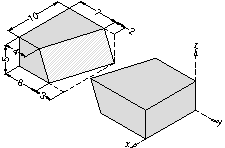
\includegraphics[width=2.5in]{Ejer3_12_3.pdf}\label{corte}}
		\hspace{1.0cm}
		\subfloat [Resistencia del pegamento.]{ 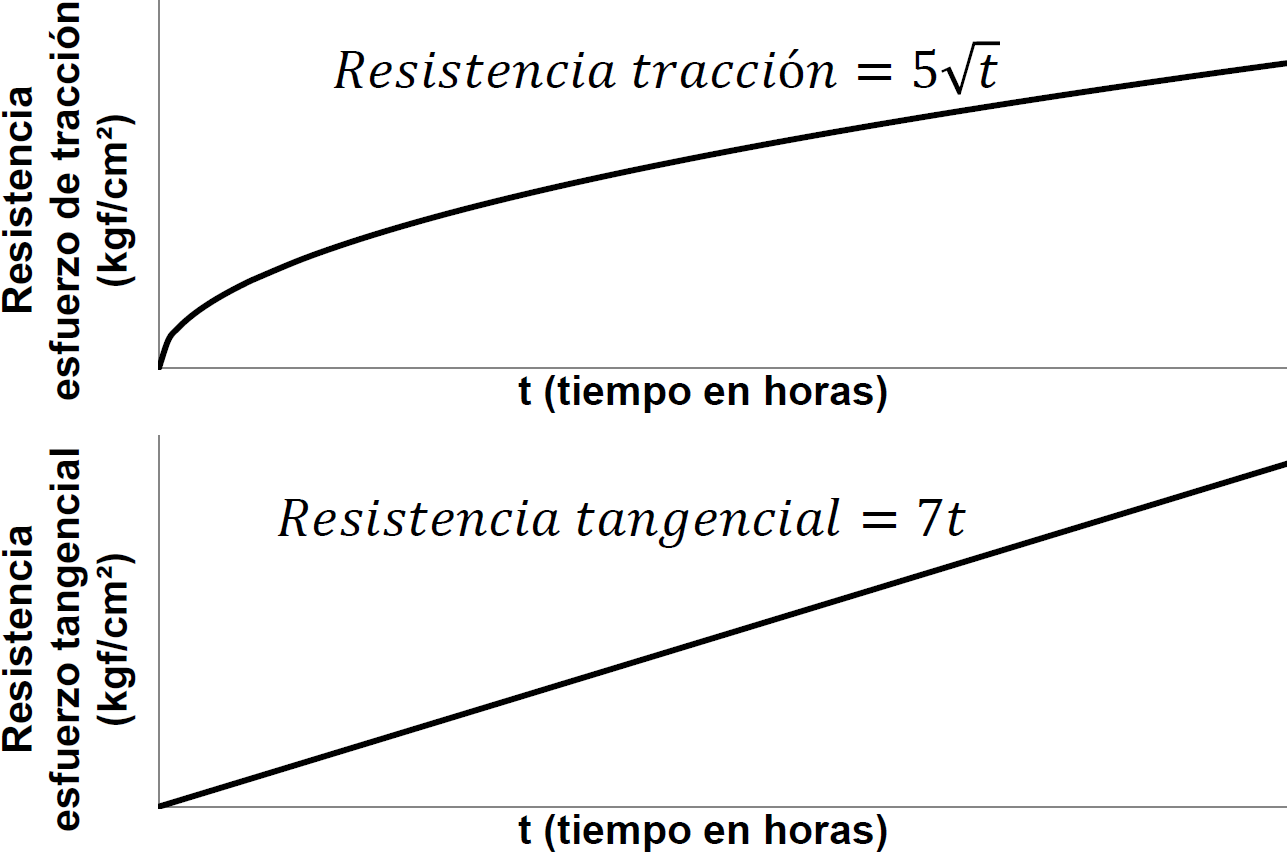
\includegraphics[width=2.5in]{Ejer3_12_4.png}\label{curvas2}}		
	\caption{ }
\end{figure}
%
\begin{enumerate}
	\item Determine cuál es el  tiempo mínimo que se debe esperar tras aplicar el pegamento para poder colocar el bloque nuevamente en el muro sin que falle.  
\end{enumerate}
%
% *************************** %
\item \label{punto13} La \cref{esta:tensiopoint} muestra el estado de
tensiones en un punto al interior de un Medio Continuo. Sobre la cara asociada al eje $y'$ se dan las tensiones $\sigma_{y'y'}$ y $\tau_{y'x'}$ y sobre la cara asociada al eje $x'$ se da el vector de tracciones expresado en el sistema de referencia $x-y$.\\
%
\begin{figure}[H]
	\centering
	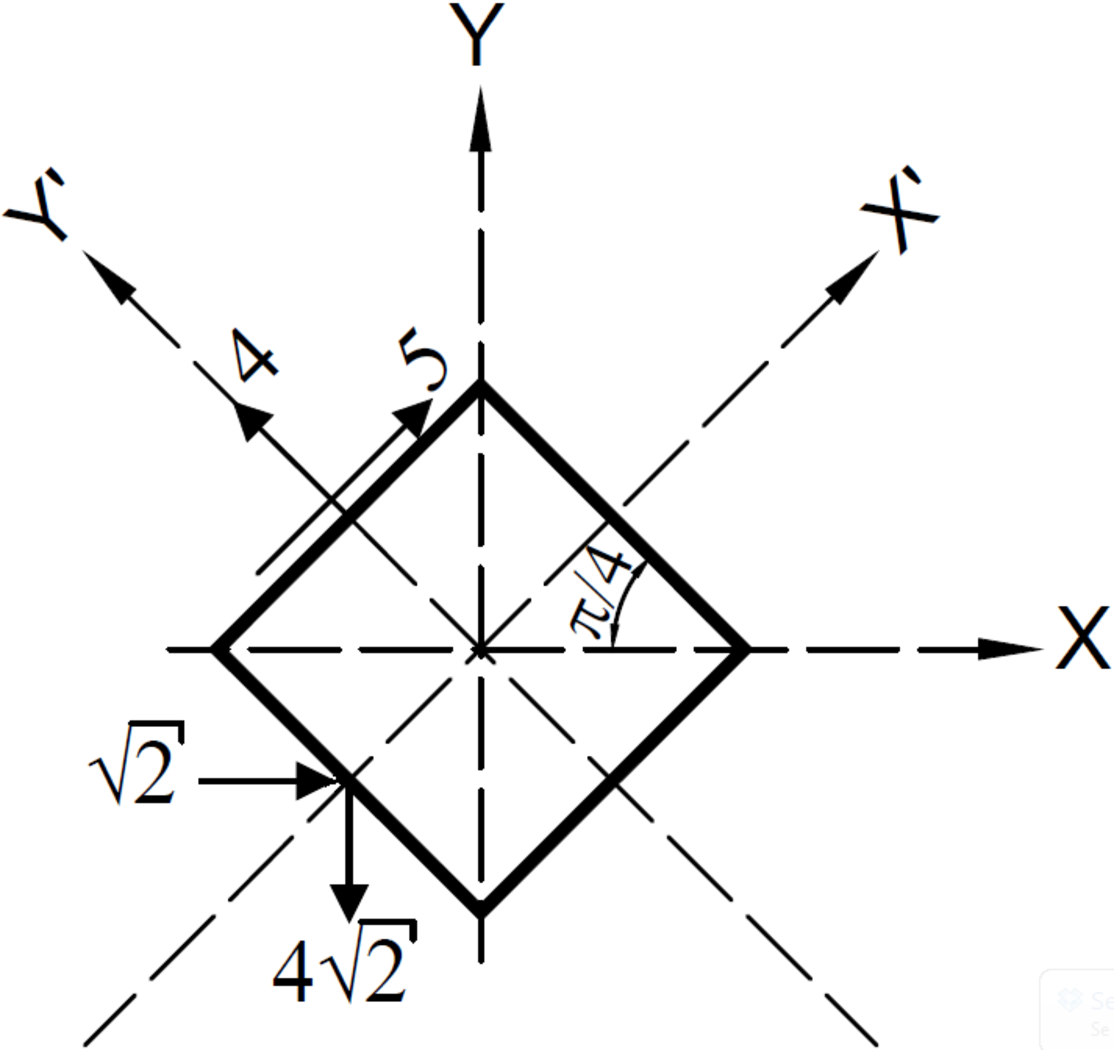
\includegraphics[height=6.25cm]{Ejer3_13.pdf}
	\caption{Estado de tensiones en un punto al interior de un medio continuo.}
	\label{esta:tensiopoint}
\end{figure}

\begin{enumerate}
	\item Escribir el tensor de tensiones en el sistema de referencia $x'-y'$.
	\item Escribir el tensor de tensiones en el sistema de referencia $x-y$.
\end{enumerate}
% *************************** %
\item \label{punto14} A continuaci\'on se presenta el tensor de esfuerzos para
un punto de un medio continuo en el sistema de referencia $x-y-z$.\\
\begin{large}
	$[\sigma] = \left[ \begin{array}{ccc}
	1 & 4 & 5 \\ 
	4 & 2 & 6 \\
	5 & 6 & 3
	\end{array}  \right] $ \\\\\\
\end{large}
%
Escriba el tensor de esfuerzos \begin{large} $\sigma'$ \end{large} asociado al
mismo punto del medio continuo pero en el sistema de referencia cuyos ejes
coordenados $x'-y'-z'$ est\'an descritos por los siguientes vectores unitarios:
\\
	$\hat{e}_{x'}= cos (\pi) \hat{i} + cos (\pi /2) \hat{j} + cos (\pi /2) \hat{k}$\\
	$\hat{e}_{y'}= cos (\pi /2) \hat{i} + cos (\pi) \hat{j} + cos (\pi /2) \hat{k}$\\
	$\hat{e}_{z'}= cos (\pi /2) \hat{i} + cos (\pi /2) \hat{j} + cos (2 \pi) \hat{k}$
% *************************** %
\item \label{punto15} La \cref{otro:esta} muestra el estado de tensiones
en un punto al interior de un Medio Continuo en el sistema de referencia $x-y$. Adicionalmente en \'esta figura se muestra el sistema de referencia $x'-y'$ que se encuentra rotado y desplazado respecto al sistema $x-y$. \textquestiondown Cu\'al de las siguientes respuestas representa correctamente el tensor en el sistema de referencia $x'-y'$?.
%
	\begin{enumerate}
		\item $[\sigma] = \left[ \begin{array}{ccc}
			a & b \\ 
			b & -c
			\end{array}  \right] $
		\item $[\sigma] = \left[ \begin{array}{ccc}
			-c & -b \\ 
			-b & a
			\end{array}  \right] $
		\item $[\sigma] = \left[ \begin{array}{ccc}
			-c-w & -b-(w+z) \\ 
			-b-(w+z) & a-z
			\end{array}  \right] $
		\item $[\sigma] = \left[ \begin{array}{ccc}
			a-w & b-(w+z) \\ 
			b-(w+z) & -c-z
			\end{array}  \right] $
		\item $[\sigma] = \left[ \begin{array}{ccc}
			-c & b \\ 
			b & a
			\end{array}  \right] $

		\item Ninguno de los tensores presentados en las opciones de la $(a)$ a la $(g)$.
	\end{enumerate}
%
\begin{figure}[H]
	\centering
	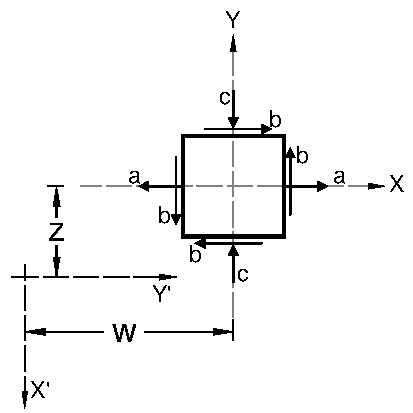
\includegraphics[height=6.0cm]{Ejer3_15.pdf}
	\caption{Estado de tensiones en un punto al interior de un medio continuo.}
	\label{otro:esta}
\end{figure}
%
% *************************** %
\item \label{punto16} Se quiere someter una columna a una tensi\'on de
compresi\'on uniforme de $100\hspace{.15cm} kgf/cm^2$ en su superficie superior, ver la  \cref{ColComp}, y se dispone s\'olo de cinco materiales diferentes cuyas capacidades m\'aximas se relacionan en el cuadro \cref{tab:materiales}:
%
\begin{figure}[H]
	\centering
		\subfloat [Columna sometida a una tensi\'on de compresi\'on $\sigma_{yy}$.]{ 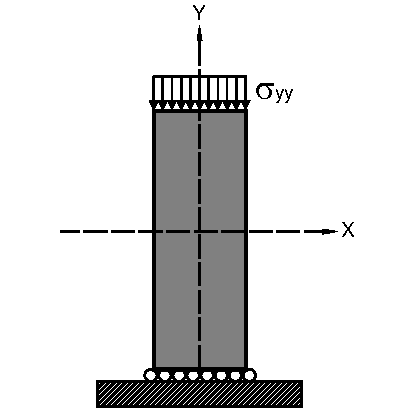
\includegraphics[width=2.5in]{Ejer3_16_1.pdf}\label{Bloq_corte}}
		\hspace{1.0cm}
		\subfloat [Tensor de tensiones en cualquier punto al interior de la columna.]{ 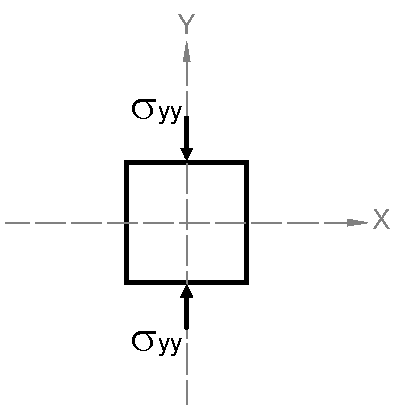
\includegraphics[width=2.5in]{Ejer3_16_2.pdf}\label{curvas}}		
	\label{ColComp}
	\caption{Columna sometida a carga vertical en la parte superior}
\end{figure}
%
\begin{table}[H]
\small
\center
    \begin{tabular}{p{4cm} c  c  c  c   c }
     & Material 1 & Material 2 & Material 3 & Material 4 & Material 5 \\  \hline
    Capacidad M\'axima a Cortante & $40$ & $60$ & $40$ & $160$ & $50$\\
    Capacidad M\'axima a Tracci\'on & $100$ & $60$ & $10$ & $20$ & $10$\\ 
    Capacidad M\'axima a Compresi\'on & $120$ & $60$ & $110$ & $80$ & $80$\\ 
   \end{tabular}
\caption {Esfuerzos m\'aximos soportados por los materiles en $kgf/cm^2$.} \label{tab:materiales} 
\end{table}
%

Determine con cual o cuales materiales se puede construir la columna sin que se produzca la falla.
%
% *************************** %
\item \label{punto17} En las \cref{viga:empo} y  \cref{viga:emp2}  se
muestra una viga empotrada en su extremo izquierdo y sometida a cargas distribuidas, $a$,  y $b$, respectivamente, sobre las caras indicadas.\\
%
\begin{figure}[H]
	\centering
		\subfloat [Viga sometida a carga distribuida $a$.]{ 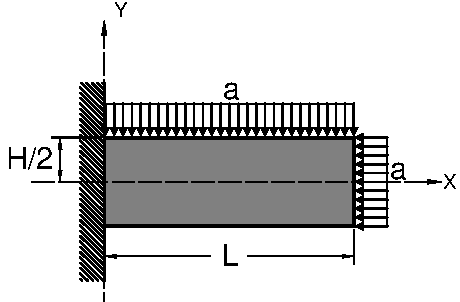
\includegraphics[width=2.5in]{Ejer3_17_1.pdf}\label{viga:empo}}
		\hspace{2.0cm}
		\subfloat [Viga sometida a carga distribuida $b$.]{ \includegraphics[width=2.5in]{Ejer3_17_2.pdf}\label{viga:emp2}}		
	\caption{ }
\end{figure}
%
Se quiere estudiar los esfuerzos en el punto de coordenadas ($L,H/2$), para lo cual se pide:

\begin{enumerate}
	\item Para cada uno de las vigas y sobre los cortes mostrados en la \cref{colme:1} indicar la direcci\'on y el valor del esfuerzo normal y tangencial sobre las 6 caras presentadas. 
	\item Para cada uno de las vigas calcule los vectores de tracciones en el sistema de referencia $ X Y$ sobre las 6 caras indicadas, e il\'ustrelos completamente en la \cref{colme:2}
\end{enumerate}

\begin{figure}[H]
	\centering
		\subfloat [Punto ($L,H/2$). Presentar esfuerzos normales y tangenciales.]{ \includegraphics[width=2.5in]{Ejer3_18.pdf}\label{colme:1}}
		\hspace{2.0cm}
		\subfloat [Punto ($L,H/2$). Presentar vectores de tracciones en $x-y$.]{ \includegraphics[width=2.5in]{Ejer3_18.pdf}\label{colme:2}}		
	\caption{ }
\end{figure}

% *************************** %
\item \label{punto18} Si el tensor de esfuerzos en un punto $P$, en el sistema
de referencia $X,Y,Z$ est\'a definidido por:\\\\
\hspace*{10mm} $ \sigma_{xx} = 80\dfrac{kgf}{cm^2}$ \hspace*{5mm} ;   \hspace*{5mm} $\sigma_{yy} = 50\dfrac{kgf}{cm^2}$\hspace*{5mm} ;\hspace*{5mm} $\sigma_{zz} = 60$ $\dfrac{kgf}{cm^2}$\\\\
\\
	\hspace*{10mm}  $ \tau_{xy} = \tau_{yx} =40\dfrac{kgf}{cm^2}$ \hspace*{5mm}; \hspace*{5mm}$\tau_{xz} = \tau_{zx} =30\dfrac{kgf}{cm^2}$\hspace*{5mm} ;\hspace*{5mm} $\tau_{yz} = \tau_{zy} = 10 \dfrac{kgf}{cm^2}$\\\\	
\\	
Y las coordenadas de los puntos $A$, $B$ y $C$  en el sistema de referencia $X,Y,Z$  son   $(1,0,0)$ , $(0,2,0)$ y $(0,0,3)$  respectivamente. Se pide lo siguiente:

\begin{enumerate}
	\item Calcular el vector de tracciones $\vec{t}$, que act\'ua en la cara del punto $P$, que es paralela al plano que contiene  los puntos $A$ , $B$ y $C$.
	\item Calcular el esfuerzo normal al que est\'a sometida la cara del punto $P$, que es paralela al plano que contiene los puntos $A$ , $B$ y $C$.
	\item Calcular la magnitud del esfuerzo tangencial al que est\'a sometida la cara del punto $P$, que es paralela al plano que contiene los puntos $A$ , $B$ y $C$.
	\item Encontrar la matriz de transformaci\'on del sistema de referencia $X-Y-Z$ al sistema de referencia $X'-Y'-Z'$ para el cual el eje $X'$ es paralelo al vector $\vec{V}_{AB}$ y el eje $Y'$ es normal al vector normal al plano que contiene los puntos A, B y C.\\
\end{enumerate}
%	
\item \label{punto19} El estado de esfuerzos en un punto de un medio continuo
est\'a dado por:\\\\
%
\hspace*{10mm} $ \sigma_{xx} (t)= 0.0$\hspace*{5mm} \hspace*{5mm}; $\sigma_{yy} (t) = K(t)$ \hspace*{5mm};\hspace*{5mm} $ \tau_{xy} (t) = \tau_{yx} (t) =-\dfrac{K(t)}{2.0}$ \\
\\	
%
Donde, $K(t)$ es un par\'ametro que var\'ia en funci\'on del tiempo $t$, tal como se muestra en la gr\'afica y tabla presentadas en la \cref{curva:carga}. \\
%
\begin{figure}[H]
\centering
\includegraphics[height=6cm]{Ejer3_19.pdf}
\caption{Variaci\'on del parametro $K$}
\label{curva:carga}
\end{figure}
%
\begin{enumerate}
	\item Si el material es infinitamente resistente ante esfuerzos normales (axiales), pero no soporta esfuerzos cortantes mayores o iguales a $12\dfrac{kgf}{cm^2}$ determine el instante en que se presenta la falla en caso de que se presente. Si no hay falla ind\'iquelo claramente.
%
	\item Si el material \'unicamente soporta esfuerzos tangenciales menores a 15 $\dfrac{kgf}{cm^2}$, esfuerzos de compresi\'on menores a 3 $\dfrac{kgf}{cm^2}$, y esfuerzos de tracci\'on menores a 20 $\dfrac{kgf}{cm^2}$ determine el instante en que se presenta la falla en caso de que se presente. Si no hay falla ind\'iquelo claramente. \\
\end{enumerate} 
%
% *************************** %
\item \label{punto20} En la \cref{piramide} se presentan tres planos asociados a un punto $P$ de un Medio Continuo.
%
\begin{figure}[H]
	\centering
		\subfloat []{ \includegraphics[width=2.5in]{Ejer3_20_1.pdf}\label{piramide}}
		\hspace{2.0cm}
		\subfloat []{ \includegraphics[width=2.3in]{Ejer3_20_2.pdf}\label{plano45}}		
	\caption{Planos de corte en el medio continuo}
\end{figure}
%
 Si se tiene conocen tres vectores de tracciones dados por: $\overset{\rightarrow} t _{1}= \dfrac{3 \sqrt{2}}{2} \hat{i} + 4 \sqrt{2} \hat{j} + 5 \sqrt{2} \hat{k}$ , $\overset{\rightarrow} t _{2}= \dfrac{\sqrt{2}}{2} \hat{i} + 2 \sqrt{2} \hat{j} -  \sqrt{2} \hat{k}$, 
$\overset{\rightarrow} t _{3}= 4 \hat{i} + 1 \hat{j} + 2 \hat{k}$; determine el tensor de tensiones $ \left[ \sigma \right] $, en el sistema de referencia $x-y-z$, que proyectado sobre los planos con vectores normales $\hat{n}_{1}$, $\hat{n}_{2}$ y $\hat{n}_{3}$ genera los vectores de tensiones $\overset{\rightarrow} t _{1}$, $\overset{\rightarrow} t _{2}$ y $\overset{\rightarrow} t _{3}$. Los vectores $\hat{n}_{1}$ y $\hat{n}_{2}$ se encuentran contenidos en el plano $z-y$, tal como se muestra en la \cref{plano45} y $\hat{n}_{3}=1 \hat{i}$.

\item \label{punto21} El tensor de tensiones en el punto $P$ está definido
como
%	
\begin{large}
	\[ [\sigma] = \left[ \begin{array}{ccc}
	F & G & -H \\ 
	G & 3F & 2G \\ 
	-H & 2G & -F
	\end{array}  \right] \enspace\]
\end{large}
%
Calcular el vector de tracción en el punto $P$ seg\'un la normal al plano definido por los puntos $A$, $C$ y el origen del sistema de referencia (ver \cref{vecplano}). Descomponer en componentes tangenciales y normal a dicho plano.
\begin{figure}[H]
	\centering
	\includegraphics[width=5 cm]{Ejer3_21.pdf}
	\vspace{-.5 cm}
	\caption{}
	\label{vecplano}
\end{figure}

\item \label{punto22} Para el medio continuo mostrado  en la \cref{MedioCon}
se sabe que el tensor de esfuerzos asociado a un sistema de referencia $xy$ y debido a la acción de una carga $P_1$ (\cref{sisxy}) está dado por $[\sigma]$; y el tensor  de esfuerzos asociado a un sistema de referencia $x'y'$ y debido a la acción de una carga $P_2$ (\cref{sisxpyp})  está dado por un tensor $[\sigma']$. Ambos sistemas de referencia comparten el origen, pero se encuentran rotados uno respecto al otro.
%
\begin{figure}[H]
	\centering
		\subfloat [Carga $P_1$ y punto en el sistema de referencia $xy$]{ \includegraphics[width=2.5in]{Ejer3_22_1.pdf}\label{sisxy}}
		\hspace{2.0cm}
		\subfloat [Carga $P_2$ y punto en el sistema de referencia $x'y'$.]{ \includegraphics[width=2.5in]{Ejer3_22_2.pdf}\label{sisxpyp}}		
	\caption{ Medio Continuo}
	\label{MedioCon}
\end{figure}

Se tiene que $[\sigma]$, en el sistema de referencia $xy$ y debido a la carga $P_1$, es igual a
\[[\sigma] = \dfrac{2P_1}{\pi} \left[ \begin{array}{ccc}
- \dfrac{x^3}{\left(x^2+y^2 \right)^2} &  \dfrac{yx^2}{\left(x^2+y^2 \right)^2}\\ \\
 \dfrac{yx^2}{\left(x^2+y^2 \right)^2} &- \dfrac{xy^2}{\left(x^2+y^2 \right)^2}\\
\end{array}  \right]\]
 
Y $[\sigma']$, en el sistema de referencia $x'y'$ y debido a la carga $P_2$, es igual a
 \[[\sigma'] = \left[ \begin{array}{ccc}
0.5 & 1.5\\ \\
1.5 & 4.5\\
\end{array}  \right]\]

Si se quiere estudiar el punto A y se sabe que el valor de la carga $P_1$ es $P_1= 25.0$,  y las coordenadas  en el sistema de referencia $xy$ del punto a estudiar corresponden a $x=\dfrac{1.0}{\pi}$, $y=\dfrac{2.0}{\pi}$, entonces:
\begin{enumerate}
	\item Encuentre los esfuerzos axiales máximos asociados a $[\sigma]$ y
	$[\sigma']$ de forma independiente
	\item Determine el ángulo entre el sistema de referencia $xy$ y el sistema de
	referencia primado $x'y'$ (ángulo entre el eje $x$ y $x'$). Se sabe que el
	ángulo conformado entre la dirección dónde se presenta el esfuerzo máximo a
	compresión del tensor  $[\sigma]$, y la dirección asociada al esfuerzo máximo a tracción del tensor $[\sigma']$ es $0.0^{\circ}$.
	\item Si se considera que el estado de esfuerzos en un medio continuo está
	descrito por la superposición de los efectos de las cargas $P_1$ y $P_2$,
	tensores $[\sigma]$ y $[\sigma']$, determine el esfuerzo tangencial (cortante)
	máximo al que está sometido el punto.
\end{enumerate}

\item \label{punto23} Un medio continuo es sometido al estado de cargas externas  mostrado en la \cref{ensayo}. Estas cargas producen un estado de esfuerzos en todos los puntos  al interior del cuerpo  representado  por la \cref{tensor}. 
	%
\begin{figure}[H]
	\centering
		\subfloat [Elemento sometido a cargas perimetrales]{ \includegraphics[width=2.5in]{Ejer4_23_1.pdf}\label{ensayo}}
		\hspace{2.0cm}
		\subfloat [Tensor de esfuezos]{ \includegraphics[width=2.5in]{Ejer4_23_2.pdf}\label{tensor}}		
	\caption{ Medio Continuo}
\end{figure}

Si el criterio de falla del material está dado por: $\tau = \sigma + 2.0 \;\; (kgf/cm^2)$ y  la carga externa $P$ es aumentada mediante la relación $P = Kt + 6.0$, con $K > 0$ y $P$ es dado en $ (kgf/cm^2)$   . Determine: 

\begin{enumerate}
\item El valor máximo de la carga  $P$ que puede ser aplicada antes que se produzca la  falla en el elemento.
\item El tiempo $t$ en el que se presenta la falla.
\item La  dirección del plano en que se produce la falla del elemento.  
\item El valor y la dirección del cortante máximo al que está sometido el punto en el momento de la falla. 
\end{enumerate}

\item \label{punto24} Dado el siguiente tensor de esfuerzos asociado a un punto
de un medio continuo:
	%
\[ [\sigma] = \left[ \begin{array}{ccc}
	5 & 0 & 0 \\ 
	0 & 4 & 0 \\ 
	0 & 0 & 3
	\end{array}  \right] \enspace \]
		%
	\begin{enumerate}
		\item Encuentre las direcciones principales del tensor.
		\item Encontrar el valor cortante máximo.
		\item Encontrar las direcciones en las cuales se presenta el cortante máximo.
		\item Determinar el valor del cortante mínimo y direcciones en las cuales se presenta el cortante mínimo.
	\end{enumerate}
% **************** %
 \item \label{punto25} El estado de tensión en un punto $P$ del Medio Continuo
se da en la \cref{cubo}. \footnote{Tomado del ejemplo 3.5 en Olivella, X; Saracíbar, C (2000). Mecánica de Medios Continuos para ingenieros}\\
%
\begin{figure}[H]
	\centering
	\includegraphics[width=8cm]{Ejer4_8.pdf}
	\caption{Estado de tensiones en el punto.}
	\label{cubo}
\end{figure}

Se pide:
	\begin{enumerate}
		\item Determinar el valor de la componente $\sigma_{22}$ del tensor de tensiones para que exista al menos un plano que pase por $P$ que est\'e libre de tensiones.
		%
		\item Determinar el vector normal a dicho plano.
		%
		\item Determinar los esfuerzos axiales máximos correspondientes al estado de tensiones presentado.
		%
		\item Determinar las direcciones principales del tensor de esfuerzo.
		%
		\item Determinar la matriz de transformación entre el sistema de referencia $x1-x2-x3$ y el que es colineal con las direcciones pricipales.
		%
		\item Determinar el máximo valor del esfuerzo cortante.
		%
	\end{enumerate}
	
\item  \label{punto26}  A continuación se presenta el tensor de esfuerzos
para un mismo punto de un medio continuo en los sistemas de referencia $x-y-z$ y $x'-y'-z'$.\\
	%
	\\
	$[\sigma] = \left[ \begin{array}{ccc}
	1/2 & 1 & 3/2 \\ 
	1 & 2 & 3 \\
	3/2 & 3 & 1/2
	\end{array}  \right] $
	\hspace{30mm}
	$[\sigma'] = \left[ \begin{array}{ccc}
	A-2 & 0 & 0 \\ 
	0 & A & 0 \\
	0 & 0 & 5
	\end{array}  \right] $
	%
	\begin{enumerate}
		\item Determine el valor de A.
		\item ¿Cuál es el valor del esfuerzo máximo a compresión que se presenta en el punto?. Determine la dirección con respecto al sistema de referencia x-y-z en donde dicho esfuerzo se presenta. 
		\item ¿Cuál es el valor del esfuerzo máximo a tracción que se presenta en el punto?. Determine la dirección con respecto al sistema de referencia x-y-z en donde dicho esfuerzo se presenta. 
		\item Determine el vector de tracciones respecto al sistema de referencia x-y-z en la cara en la que se presenta el esfuerzo máximo a compresión.
		\item Determine el vector de tracciones respecto al sistema de referencia x-y-z en la cara en la que se presenta el esfuerzo m\'aximo a tracción.
		\item Escriba el tensor en el sistema de referencia conformado por las direcciones principales.
		\item Cual es la magnitud del máximo esfuerzo cortante que puede experimentar el punto.  \\
	\end{enumerate}
\end{enumerate}

\end{document}